\documentclass{article}
\usepackage{graphicx} % Required for inserting images
\usepackage{ctex}
\usepackage{amsmath, amsthm, amssymb, bm, color, framed, graphicx, hyperref, mathrsfs}
\usepackage{geometry}
\geometry{left=2cm,right=2cm,top=2cm,bottom=2cm}
\everymath{\displaystyle}
\title{\textbf{数学分析III:级数}}
\author{南京审计大学\hspace{0.5cm}赵鸿霏}
\date{\today}
\linespread{1.5}
\newtheorem{definition}{定义}[subsection]
\newtheorem{theorem}{定理}[subsection]
\newtheorem{proposition}{命题}[subsection]
\newtheorem{example}{例}[subsection]
\newtheorem{problem}{习题}[subsection]
\newtheorem{note}{注}[subsection]
\newtheorem{lemma}{引理}[subsection]
\newtheorem{corollary}{推论}[subsection]
\newtheorem{question}{问题}[subsection]
\begin{document}
\maketitle
\tableofcontents
\newpage
\begin{center}
\begin{huge}
     \textbf{前言}
\end{huge}
\end{center}
我们先将主要的参考书罗列如下:\par
1. 徐森林《数学分析》:这是中国科学技术大学的经典数分教材之一(另一本是史济怀),特点是堆砌了相当多的内容,对很多问题的处理也比较古典。但也正是因为堆砌,所以内容比较全面,我们的很多古典的定理以及证明都来自这本书。\par
2. 梅加强《数学分析》:这是南京大学的数分教材。梅加强老师是做几何的,所以这本书的几何味道很重。这本书是我看多元时候的主要参考书,里面讲了一些观点现代的东西,值得一看。\par
3. 谢惠民《数学分析习题课讲义》:这可以说是当今市面上最好的数学分析习题书(没有之一)。我们的很多习题材料都取材于这本书。这本书的下册比较偏重后续课程,例如在级数部分介绍了Fourier分析中的东西(我们也会涉及到一些),在多元微积分中介绍了微分形式等,这是现代几何学中相当有用的内容。\par
4. 克莱因《古今数学思想》:我们的很多有趣的(希望如此)小故事来自这本书。\par
5. 艾格纳、齐格勒《数学天书中的证明》:这本书记载了一些问题的优美的证明。我们的一些习题资料取材于这本书。\par
6. 鲁金《实变函数论》:我们参考了这本书介绍的无穷函数项级数中一致收敛的引入动机,以及其中的一些例子。\par
7. 汪林《数学分析中的反例》:我们的反例大多来自于这本书。\par
8. 张恭庆《泛函分析讲义》第二版上册:我们对Arzela-Ascoli定理的证明取材于这里。\par
9. 夏道行《实变函数与泛函分析基础》:我们引用的Helly选取原理的证明来自这本书。\par
10. Munkres \textit{Topology}: 我们的Baire纲定理与一些拓扑术语来自这本书。\par
这份讲义的内容并没有什么修饰,它粗略地记录了笔者在2023年暑期线上讨论课上介绍级数的一些内容。事实上更多的补充内容并没有包含在正文中,其本身也没有什么原创性。事实上笔者确切的知道这份讲义中有一些笔误和没有写完(烂尾)的部分,至于没有重写或者修订的原因,一个是讲义中绝大多数内容都可以在主流数分教材中找到,另一个原因是笔者太懒。由于笔者水平有限,再加上时间仓促,讲义中定会有大量尚未发现的笔误甚至错误,欢迎读者通过QQ:422276215反馈。
\begin{flushright}
    \begin{tabular}{c}
        赵鸿霏\\
        南京审计大学\\
        \today
    \end{tabular}
\end{flushright}
\newpage
\section{无穷级数}
\subsection{数项级数}
无穷级数在数学中的出现是很早的,早期的无穷级数出现的形式通常是公比小于$1$的无穷几何级数,即:
$$\sum_{n=1}^\infty q^n,0<q<1.$$
早在古希腊时期亚里士多德就认识到这种级数有和。无穷级数还散见在中世纪后期的一些数学家的著作中,例如早在(约)1360年,数学家奥雷姆在他的小册子《欧几里得几何问题》中就证明了调和级数
$$1+\frac{1}{2}+\frac{1}{3}+\frac{1}{4}+\cdots$$
是发散的。\par
时间来到17世纪中叶,墨卡托和牛顿发现了级数
$$\ln(1+x)=x-\frac{1}{2}x^2+\frac{1}{3}x^3+\cdots,$$
我们很快发现这就是$\ln(1+x)$的泰勒展开式。然而人们观察到,如果我们令$x=3$,那么上式左面有值,但右面却发散。沃利斯注意到了这个困难,但不能解释它。这启示我们级数的理论尚有许多工作要做,而本章我们就将介绍当时的数学家在这方面做出的努力。\par
我们首先给出级数的一般化定义。
\begin{definition}
设$a_1,a_2,\cdots,a_n,\cdots$为一实数列,称形式和$\sum_{n=1}^\infty a_n$
为\textbf{无穷级数},其中$a_n$称为该无穷级数的\textbf{第$n$项},称$S_n=\sum_{k=1}^na_k$
为该无穷级数的\textbf{部分和}或\textbf{前$n$项和}。如果
$$\lim_{n\to\infty}S_n=\lim_{n\to\infty}\sum_{k=1}^na_k=S\in\mathbb{R},$$
就称该数项级数\textbf{收敛},并记$\sum_{n=1}^\infty a_n=S,$否则称该数项级数\textbf{发散}。
\end{definition}
请注意:这里的$\sum_{n=1}^\infty a_n$还仅仅是一个形式记号,即我们不知道它是否有意义。但根据上述定义,我们已经把讨论级数收敛与否的问题转化成了一个序列极限的问题,而这是为我们所熟知的。
\begin{example}
我们现在来介绍奥雷姆证明调和级数发散的方法。他注意到
$$
1+\frac{1}{2}+\frac{1}{3}+\frac{1}{4}+\frac{1}{5}+\frac{1}{6}+\frac{1}{7}+\frac{1}{8}+\cdots >\left( \frac{1}{2}+\frac{1}{2} \right) +\left( \frac{1}{4}+\frac{1}{4} \right) +\left( \frac{1}{8}+\frac{1}{8}+\frac{1}{8}+\frac{1}{8} \right) +\cdots ,
$$
从而如果我们记
$$
H_n=1+\frac{1}{2}+\frac{1}{3}+\frac{1}{4}+\frac{1}{5}+\frac{1}{6}+\frac{1}{7}+\frac{1}{8}+\cdots ,
$$
就有
$$
H_n>1+\frac{1}{2}+\frac{1}{2}+\frac{1}{2}+\cdots 
$$
而后者显然发散。
\end{example}
\begin{example}(芝诺的乌龟)
阿喀琉斯是古希腊有名的善跑的英雄。假设阿喀琉斯和乌龟进行赛跑,其速度是乌龟的10倍。芝诺说:阿喀琉斯永远也追不上乌龟,因为乌龟每行100米,阿喀琉斯就要向前追100米,而在这个过程中乌龟又向前行了10米,于是阿喀琉斯又要向前追10米,而这个过程中乌龟又向前行了1米......芝诺提出这个悖论来支持他的老师巴门尼德的关于“存在”不动、是一的学说。\par
时间来到17世纪中叶,圣文森特的格雷戈里在他的《几何著作》中,证明了追乌龟的悖论可以用几何级数的求和来解决。即注意到$\sum_{n=1}^{\infty}{\frac{1}{10^n}}<\infty $. 他说:“过程的结束就是级数的终点,即使延续到无穷,过程也永远达不到这个终点,但是它能够趋向于并接近到任何给定的程度”。他对这个课题做出的贡献影响了很多学生。
\end{example}
\begin{example}
在高中阶段我们介绍过很多求和手段,对于大家十分熟悉的结构我们不再列出。下面介绍几个(高中阶段可能)不那么常见的求和技巧。\par
1. 求$\sum_{n=1}^{\infty}{\arctan \frac{1}{n^2+n+1}}$. 利用公式
$$
\arctan a-\arctan b=\arctan \frac{a-b}{1+ab},
$$
我们有
$$
\sum_{n=1}^{\infty}{\arctan \frac{1}{n^2+n+1}}=\sum_{n=1}^{\infty}{\arctan \frac{n+1-n}{n\left( n+1 \right) +1}}=\sum_{n=1}^{\infty}{\left[ \arctan \left( n+1 \right) -\arctan n \right]}=\lim_{n\rightarrow \infty} \arctan \left( n+1 \right) -\frac{\pi}{4}=\frac{\pi}{4}.
$$
2.求$\sum_{n=1}^m{\cos \left( n+1 \right)}$.注意到
$$
\sum_{n=1}^m{\cos \left( n+1 \right)}=\frac{\sum_{n=1}^m{\sin \frac{1}{2}\cos \left( n+1 \right)}}{\sin \frac{1}{2}}=\frac{\sum_{n=1}^m{\left[ \sin \left( \frac{3}{2}+n \right) -\sin \left( \frac{1}{2}+n \right) \right]}}{2\sin \frac{1}{2}}=\frac{1}{2}\csc \frac{1}{2}\left[ \sin \left( \frac{3}{2}+m \right) -\sin \frac{3}{2} \right] .
$$
事实上更一般地,我们有
$$
\sum{\text{正余弦函数}\left( \text{等差数列} \right)}=\frac{\sin \frac{\text{公差}}{2}\sum{\text{正余弦函数}\left( \text{等差数列} \right)}}{\sin \frac{\text{公差}}{2}},
$$
并利用和差化积来进行裂项。\par
3.求$\sum_{n=1}^{\infty}{r^n\sin nx}$,这里$0<r<1$. 我们利用Euler公式$z=r\left[ \cos x+\mathrm{i}\sin x \right] $就有
$$
\sum_{n=1}^{\infty}{r^n\sin nx}=\mathrm{Im}\sum_{n=1}^{\infty}{z^n}=\mathrm{Im}\frac{z}{1-z}.
$$
后续的计算细节我们不再展开。
\end{example}
我们指出:绝大多数的初等求和都可以通过软件计算(例如WolframAlpha等)来完成,因此与其进行大量的奇淫技巧的训练,不如钻研定理与命题的证明,后者才是对数学学习更重要的部分。\par
现在我们来回顾一下反常积分。至于这么做的动机,我们考察$\int_a^\infty f(x)\mathrm{d}x$. 注意到
$$
\int_a^{\infty}{f\left( x \right) \mathrm{d}x}=\sum_{k=1}^{\infty}{\int_{a+k-1}^{a+k}{f\left( x \right) \mathrm{d}x}}=\sum_{k=1}^{\infty}{a_k},a_k=\int_{a+k-1}^{a+k}{f\left( x \right) \mathrm{d}x},
$$
这暗示着反常积分与级数之间必然有着某种联系。下面请回忆:我们已经学习了反常积分。给出一个反常积分,我们如何判断它的敛散性?一些常用的方法是将被积函数与$\frac{1}{x^p}$比较,或是Abel等判别法。事实上我们将看到,在反常积分中常用的很多判别法可以毫无困难地推广到级数当中去。
\begin{theorem}
级数$\sum_{n=1}^\infty a_n$收敛当且仅当对任意的$\varepsilon>0$,存在某个$N\in\mathbb{N}$,使得当$k,m>N$时成立$\left|\sum_{n=k}^ma_n\right|<\varepsilon$.
\end{theorem}
\begin{proof}
级数$\sum_{n=1}^\infty a_n$收敛当且仅当$S_n=\sum_{i=1}^na_i$收敛。由数列的Cauchy收敛准则,即证!
\end{proof}
\begin{theorem}
设$\sum_{n=1}^\infty a_n$收敛,那么$\lim_{n\to\infty}a_n=0$,但反之不真。
\end{theorem}
\begin{proof}
由于$\sum_{n=1}^\infty a_n$收敛,因此序列$S_n=\sum_{k=1}^na_k$收敛。从而我们有
$$
\lim_{n\rightarrow \infty} a_n=\lim_{n\rightarrow \infty} \left( S_n-S_{n-1} \right) =\lim_{n\rightarrow \infty} S_n-\lim_{n\rightarrow \infty} S_{n-1}=S-S=0.
$$
反之,令$a_n=\frac{1}{n}$,则$\lim_{n\to\infty}a_n=0$,但$\sum_{n=1}^\infty\frac{1}{n}$是发散的。
\end{proof}
\begin{note}
读者也许想把这个结论和反常积分做类比,然而$\int_a^\infty f(x)\mathrm{d}x$收敛并不能推出$\lim_{x\to+\infty}f(x)=0$.一个经典的反例是$f\left( x \right) =\frac{x}{1+x^6\sin ^2x}$.
\end{note}
下面的这个引理将反常积分的结果与级数联系起来。
\begin{lemma}
设$\{a_n\}$是一列实数,在$[1,+\infty)$上定义函数$\alpha(x)$如下:设$k\ge 1$,当$x\in[k,k+1)$时定义$\alpha(k)=a_k$.那么级数$\sum_{n=1}^\infty a_n$收敛当且仅当反常积分$\int_1^\infty\alpha(x)\mathrm{d}x$收敛。
\end{lemma}
\begin{proof}
令$S(x)=\int_1^x\alpha(x)\mathrm{d}x$,令$S_n$表示级数的前$n$项和,则显然我们有
$$
S\left( x \right) =S_{n-1}+\theta a_n=S_{n-1}+\theta \left( S_n-S_{n-1} \right) =\theta S_n+\left( 1-\theta \right) S_{n-1},x\in \left[ n,n+1 \right) ,
$$
其中$\theta=x-n$.因此如果$S_n$收敛于$S$,那么对任意的$\varepsilon>0$,存在$N\in\mathbb{N}$,使得当$n>N$时成立$|S_n-s|<\varepsilon$.从而
$$
\left| S\left( x \right) -S \right|\le \theta \left| S_n-S \right|+\left( 1-\theta \right) \left| S_{n-1}-S \right|<\theta \varepsilon +\left( 1-\theta \right) \varepsilon =\varepsilon ,
$$
即证!反之若$S(x)$收敛,则由$S(n)=S_{n+1}$知$S_n$收敛,因此级数收敛,即证!
\end{proof}
有了上面的引理,我们就可以将反常积分的判别法“照搬”到级数上来,现列举如下:
\begin{theorem}
(1)(Dirichlet) 设$\{a_n\}$单调地趋于$0$,级数$\sum_{n=1}^\infty b_n$的部分和有界,那么级数$\sum_{n=1}^\infty a_nb_n$收敛。\par
(2)(Abel) 设$\{a_n\}$为单调的有界数列,级数$\sum_{n=1}^\infty b_n$收敛,那么那么级数$\sum_{n=1}^\infty a_nb_n$收敛。
\end{theorem}
\begin{proof}
由引理1.1.1的以及反常积分中的结果,即证!
\end{proof}
\begin{corollary}
(Leibniz) 设$\{a_n\}$单调地趋于$0$,则级数$\sum_{n=1}^\infty(-1)^na_n$收敛。
\end{corollary}
\begin{note}
如果读者觉得上述讨论难以理解,可以先承认这个定理,我们会在一般级数的部分通过其他方式证明这两个判别法。
\end{note}
\begin{proof}
我们用Dirichlet判别法。显然$\sum_{n=1}^\infty(-1)^n$的部分和有界,结合$\{a_n\}$单调地趋于$0$就有$\sum_{n=1}^\infty(-1)^na_n$收敛。
\end{proof}
\begin{example}
考察$\sum_{n=1}^\infty\frac{\sin nx}{n}$的敛散性。利用例1.1.3中介绍的方法,我们可以求得
$$
\sum_{k=1}^n{\sin kx}=\begin{cases}
	0,x=2k\pi ,\\
	\frac{\cos \frac{x}{2}-\cos \left( n+\frac{1}{2} \right) x}{2\sin \frac{x}{2}},x\ne 2k\pi ,\\
\end{cases}
$$
从而$\sum_{n=1}^\infty\sin nx$的部分和是有界的。又$\frac{1}{n}$单调地趋于$0$,于是由Dirichlet判别法即知$\sum_{n=1}^\infty\frac{\sin nx}{n}$收敛。
\end{example}
\begin{note}
事实上利用复变函数的知识,我们甚至可以计算出这个级数的值。
\end{note}
下面我们研究级数的简单性质。
\begin{theorem}
设$\sum_{n=1}^\infty a_n,\sum_{n=1}^\infty b_n$均收敛,那么$\sum_{n=1}^\infty ca_n,\sum_{n=1}^\infty(a_n\pm b_n)$也收敛。
\end{theorem}
\begin{proof}
对第一个,我们注意到
$$
\sum_{n=1}^{\infty}{ca_n}=\lim_{n\rightarrow \infty} \sum_{k=1}^n{ca_k}=c\lim_{n\rightarrow \infty} \sum_{n=1}^{\infty}{a_k}=c\sum_{n=1}^{\infty}{a_n},
$$
因此收敛。对第二个,我们注意到
$$
\sum_{n=1}^{\infty}{\left( a_n\pm b_n \right)}=\lim_{n\rightarrow \infty} \sum_{k=1}^n{\left( a_k\pm b_k \right)}=\lim_{n\rightarrow \infty} \left( \sum_{k=1}^n{a_k}\pm \sum_{k=1}^n{b_k} \right) =\lim_{n\rightarrow \infty} \sum_{k=1}^n{a_k}\pm \lim_{n\rightarrow \infty} \sum_{k=1}^n{b_k}=\sum_{n=1}^{\infty}{a_n}\pm \sum_{n=1}^{\infty}{b_n},
$$
即证。
\end{proof}
\begin{theorem}
级数$\sum_{n=1}^\infty a_n$中去掉有限项后不改变敛散性。
\end{theorem}
\begin{proof}
设去掉级数$\sum_{n=1}^\infty a_n$的前$m$项和后得到的新级数为$\sum_{n=m+1}^\infty a_n$,记它们的部分和分别为$S_n=\sum_{k=1}^na_k,S_n^\prime=\sum_{k=m+1}^na_k$,那么
$$
\sum_{n=1}^{\infty}{a_n}\text{敛散}\Leftrightarrow S_n\text{敛散}\Leftrightarrow S_{m+n}-S_m\text{敛散}\Leftrightarrow S_{n}^{\prime}\text{敛散}\Leftrightarrow \sum_{n=m+1}^{\infty}{a_n}\text{敛散}.
$$
\end{proof}
\begin{theorem}
若级数$\sum_{n=1}^\infty a_n$收敛,那么将级数中的项不改顺序地加括号,级数的和不发生改变。即新级数
$$
\left( a_1+a_2+\cdots +a_{n_1} \right) +\left( a_{n_1+1}+a_{n_1+2}+\cdots +a_{n_2} \right) +\cdots 
$$
也收敛,且与$\sum_{n=1}^\infty a_n$相等。
\end{theorem}
\begin{proof}
记$a_{n_i+1}+a_{n_i+2}+\cdots+a_{n_{i+1}}=y_i$,那么新级数可以表示为$\sum_{n=1}^\infty y_n$.注意到它的部分和$S_{n_1},S_{n_2},\cdots$为$\sum_{n=1}^\infty a_n$的一个子列,因此由收敛序列的子列的性质,即证。
\end{proof}
\begin{note}
该命题的逆命题并不成立。例如考虑$\sum_{n=1}^\infty(-1)^{n-1}$,这个级数是发散的(为什么?),但我们可以通过适当的加括号来使它恒为任意常数。关于这个级数还有一段趣闻:大数学家欧拉为了求出这个级数的值做了如下讨论:注意到
$$
\frac{1}{1-x}=1+x+x^2+x^3+\cdots ,
$$
因此令$x=-1$,就有
$$
\frac{1}{2}=1-1+1-1+\cdots .
$$
而今天我们知道这显然是不对的(为什么?)。
\end{note}
我们指出,只要再加一个条件就可以使得定理1.1.6的逆命题也成立。注意我们给出的反例,它的一个特别之处便是各项的值来回震荡,从而可以反复抵消部分的值。如果我们要求每个加括号内的数都是同号的,能不能使得逆命题成立呢?这就是下面的定理。
\begin{theorem}
设新级数
$$
\left( a_1+a_2+\cdots +a_{n_1} \right) +\left( a_{n_1+1}+a_{n_1+2}+\cdots +a_{n_2} \right) +\cdots 
$$
在同一个括号内有相同的符号,且该级数收敛,那么原级数$\sum_{n=1}^\infty a_n$也收敛,且这两个级数的值相等。
\end{theorem}
\begin{proof}
同样地,我们设新级数为$\sum_{n=1}^\infty y_n$.由于每一个括号内的数都是同号的,因此对于$\sum_{n=1}^\infty y_n$的部分和$S_k^\prime=S_{n_k}$与$S_{k+1}^\prime=S_{n_{k+1}}$,对于$n_{k}\le n\le n_{k+1}$,原级数的部分和只能在$S_k^\prime$和$S_{k+1}^\prime$中单调地变动,而由于新级数收敛,故$\lim_{n\to\infty}S_n^\prime=S$,从而$\lim_{n\to\infty}S_n=S$.
\end{proof}
\begin{center}
\begin{large}
\textbf{习题1.1}
\end{large}
\end{center}
\begin{problem}
计算下列级数的和:\par
(1) $\sum_{n=1}^\infty\frac{1}{n(n+1)}$;\hspace{1cm}
(2) $\sum_{n=1}^\infty\frac{1}{10^n}$;\hspace{1cm}
(3) $\sum_{n=1}^\infty\frac{2n+1}{n^2(n+1)^2}$.
\end{problem}
\begin{problem}
设级数$\sum_{n=1}^\infty na_n$收敛,证明$\sum_{n=1}^\infty a_n$也收敛。
\end{problem}
\begin{problem}\em(指数函数的构造)\par
利用实数(作为一个线性空间)上的加法和乘法,我们能够定义多项式函数:
$$
\mathbb{R} \rightarrow \mathbb{R} ,x\mapsto a_dx^d+a_{d-1}x^{d-1}+\cdots +a_1x+a_0.
$$
现在利用级数,我们做如下定义:
\begin{definition}
我们定义指数函数$\exp:\mathbb{R}\to\mathbb{R}$如下:
$$
x\mapsto \exp \left( x \right) =\sum_{k=0}^{\infty}{\frac{x^k}{k!}}.
$$
\end{definition}
首先我们必须说明$\exp$是良定的,也就是说,对任意的$x\in\mathbb{R}$,级数$\exp(x)$都是收敛的。\par
(i)证明:存在$k\in\mathbb{N}$,使得当$k>n$时成立$\left|\frac{x^k}{k!}\right|\le\frac{1}{2^k}$.\par
(ii)说明$\sum_{k\ge N}\frac{1}{2^k}$是收敛的,进而说明定义1.1.2是良定的。\par
下面我们要研究指数函数的性质。例如,我们想知道对于任意的$x,y\in\mathbb{R}$是否有$\exp(x+y)=\exp(x)\cdot\exp(y)$(换言之,我们希望证明$\exp$是$(\mathbb{R},+)$到$(\mathbb{R}_+,\times$的一个群同态)?这需要我们进一步研究双指标的级数求和。\par
我们首先严格化“双指标”的定义:
\begin{definition}
一个\textbf{双指标序列}$\{x_{ij}\}_{i,j\ge 1}$是指一个映射$F:\mathbb{Z}_{\ge 1}\times\mathbb{Z}_{\ge 1}\to\mathbb{R}$,其中$(i,j)\mapsto x_{ij}$. 一个双指标序列的\textbf{重排}$\{y_n\}_{n\ge 1}$指的是一个双射$\Phi:\mathbb{Z}_{\ge 1}\to\mathbb{Z}_{\ge 1}\times\mathbb{Z}_{\ge 1}$,我们令$y_n=x_{\Phi(n)}$,其中$\Phi(n)$是一个双指标。
\end{definition}
下面设$\sum_{n=1}^\infty a_n$和$\sum_{n=1}^\infty b_n$都是收敛的正项级数,$\{c_n\}_{n\ge 1}$是$\{a_ib_j\}_{i,j\ge 1}$的一个重排。\par
(iii) 证明:级数$\sum_{n=1}^\infty c_n$收敛,且无论采用何种重排,都有
$$
\sum_{n=1}^{\infty}{c_n}=\left( \sum_{n=1}^{\infty}{a_n} \right) \left( \sum_{n=1}^{\infty}{b_n} \right) .
$$\par
(iv) 说明上述结论对绝对收敛的级数也成立。(提示:考虑$a_n,b_n$的正部(即若$a_n>0$,则$a_n^+=a_n$,否则$a_n^+=0$,负部同理)和负部,将$\sum c_n$分成若干个级数的和)\par
(v) 证明级数形式的Fubini定理:设$\sum_{n,m\ge 1}|a_{mn}|$收敛,那么
$$
\sum_{n=1}^{\infty}{\sum_{m=1}^{\infty}{a_{mn}}}=\sum_{m=1}^{\infty}{\sum_{n=1}^{\infty}{a_{mn}}}=\sum_{m,n=1}^{\infty}{a_{mn}}.
$$\par
(vi) 证明:$\exp(x_1+x_2)=\exp(x_1)+\exp(x_2)$.\par
此外,我们还注意到一个很简单但很重要的事实:$\exp(0)=1$(这可以直接用定义得到),利用这个事实我们可以证明下面的性质:\par
(vii) 证明:$\exp(x)\ne 0$.进一步说明$\exp(x)>0$.\par
(viii) 证明:$\exp(x)$是单调递增的函数。特别地,$\exp(x)$是单射。
\end{problem}
\begin{note}
(1) 这就是所谓的“法式风格”的习题,读者可以明显感觉到它的独特风格。至于对这种类型习题的评价,则仁者见仁智者见智了。对于不喜欢或不适应这类风格的读者可以直接寻找有关文献阅读。\par
(2) 后面我们将证明$\exp(x)$还是一个满射,从而可以定义函数$\log$.\par
(3) 我们注意到上面指数函数的定义可以推广到复数域上,进而我们可以定义三角函数:
$$
\cos z=\frac{e^{\mathrm{i}z}+e^{-\mathrm{i}z}}{2},\sin z=\frac{e^{\mathrm{i}z}-e^{-\mathrm{i}z}}{2\mathrm{i}}.
$$
在此我们不详细展开。\par
(4) 应当说,本题中一个重要的部分就是所谓的“求和换序”的处理。我们将在实分析中进一步讨论这些问题。应当指出,18世纪的数学家对于级数的处理是相当“放荡”的,他们拒绝一切严谨性的讨论而胡乱地使用级数,尽管他们的工作也产生了一些很有用的结果。事实上,坚持只能用收敛级数的主张,是经历了大半个19世纪才取得成功的。但是18世纪的人们最终还是得到了谅解:他们预见到关于无穷级数的两个很有生命力的思想,后来得到了承认。第一个是发散级数可以用来做数值逼近,第二个是级数可以在解析运算中代表函数,即使这个级数是发散的。
\end{note}
\subsection{正项级数判别法}
这一节我们主要研究正项级数。为此,我们先严格地给出正项级数的定义:
\begin{definition}
设级数$\sum_{n=1}^\infty a_n$满足对任意的$n\in\mathbb{N}_+$都有$a_n\ge 0$,则称$\sum_{n=1}^\infty a_n$为\textbf{正项级数}。特别地,若$a_n>0$,则称$\sum_{n=1}^\infty a_n$为\textbf{严格正项级数}。
\end{definition}
关于严格正项级数,一个基本的(重要的)观察如下:
\begin{proposition}
正项级数$\sum_{n=1}^\infty a_n$收敛当且仅当其部分和$S_n$有界。
\end{proposition}
\begin{proof}
必要性。设正项级数$\sum_{n=1}^\infty a_n$收敛,那么$\lim_{n\to\infty}S_n=S$.由极限的保号性知$S_n$有界。\par
充分性。设$S_n$有界,由于$\sum_{n=1}^\infty a_n$是正项级数,因此$S_n$单调。由数列极限的性质知$S_n$有极限,从而$\sum_{n=1}^\infty a_n$收敛。
\end{proof}
下面我们介绍正项级数的一些判别法。
\begin{theorem}(Cauchy)
设$f(x)$是定义在区间$[a,+\infty)$上的单调递减函数,那么反常积分$\int_a^\infty f(x)\mathrm{d}x$与级数$\sum_{n=1}^\infty f(a+n)$同敛散。
\end{theorem}
\begin{proof}
易知$\int_a^\infty f(x)\mathrm{d}x=\sum_{n=1}^\infty\int_{a+k-1}^{a+k}f(x)\mathrm{d}x$.利用$f(x)$的单调性我们有
$$
\int_{a+n-1}^{a+n}{f\left( a+n \right) \mathrm{d}x}\le \int_{a+n-1}^{a+n}{f\left( x \right) \mathrm{d}x}\le \int_{a+n-1}^{a+n}{f\left( a+n-1 \right) \mathrm{d}x},
$$
因此
$$
\sum_{n=1}^{\infty}{f\left( a+n \right)}\le \sum_{n=1}^{\infty}{\int_{a+n-1}^{a+n}{f\left( x \right) \mathrm{d}x}}=\int_a^{\infty}{f\left( x \right) \mathrm{d}x}\le \sum_{n=1}^{\infty}{f\left( a+n-1 \right)}=\sum_{n=0}^{\infty}{f\left( a+n \right)},
$$
从而级数$\sum_{n=1}^\infty f(a+n)$可以从两边控制住$\int_a^\infty f(x)\mathrm{d}x$,因此它们同敛散。
\end{proof}
\begin{note}
我们使用了一个对大家而言可能相对陌生的词:“控制”。事实上大家可以回忆反常积分的比较判别法,例如我们想判断积分$\int_2^\infty\frac{1}{x^2+1}\mathrm{d}x$收敛与否,一个自然的想法是注意到$\frac{1}{x^2+1}<\frac{1}{x^2}$,进一步我们可以应用$\frac{1}{x^2}$的性质。这里的$\frac{1}{x^2}$就是\textbf{控制函数}。如果某个控制函数可以“从两边分别控制”给定函数,那么自然它们会具有某些相同的性质,例如这里体现的是敛散性(某种有界性)。这是一种相当常用的思想。例如我们将看到在后面介绍的控制收敛定理,以及泛函分析中刻画算子间的等价性时它的威力所在。
\end{note}
\begin{example}
一个立即的推论就是\textbf{Riemann-$\zeta$}函数$\zeta(x)=\sum_{n=1}^\infty\frac{1}{n^x}$在$x\in\mathbb{R}$时的敛散性。它在$x>1$时收敛,而在$x\le 1$时发散。大名鼎鼎的Riemann猜想就是关于这个函数(在复平面上的解析延拓)的零点分布猜想。我们将在乘积级数部分进一步讨论这个函数的一些性质(当然,我们并不会证明黎曼猜想。感兴趣的读者可以自行尝试证明)。
\end{example}
\begin{example}
我们讨论级数$\sum_{n=3}^{\infty}{\frac{1}{n^{\alpha}\ln ^{\beta}n\ln ^{\gamma}\ln n}}$的敛散性。熟知当$\alpha>1$时$\int_3^{\infty}{\frac{\mathrm{d}x}{x^{\alpha}}}$收敛,当$\alpha\le 1$时$\int_3^{\infty}{\frac{\mathrm{d}x}{x^{\alpha}}}$发散。因此我们就$\alpha>1,\alpha=1,\alpha<1$分别讨论。\par
当$\alpha>1$时,不妨设$\alpha=1+2\varepsilon$,这里$\varepsilon>0$.那么
$$
\frac{1}{n^{\alpha}\ln ^{\beta}n\ln ^{\gamma}\ln n}=\frac{1}{n^{1+\varepsilon}}\cdot \frac{1}{n^{\varepsilon}\ln ^{\beta}n\ln ^{\gamma}\ln n}.
$$
注意到(利用反常积分的比较审敛法):
$$
\lim_{x\rightarrow +\infty} {{\left( \frac{1}{x^{1+\varepsilon}} \right)}\Bigg/{\left( \frac{1}{x^{\alpha}\ln ^{\beta}x\ln ^{\gamma}\ln x} \right)}}=\lim_{x\rightarrow +\infty} \frac{1}{x^{\varepsilon}\ln ^{\beta}x\ln ^{\gamma}\ln x}=0,
$$
因此$\int_3^{\infty}{\frac{\mathrm{d}x}{x^{\alpha}\ln ^{\beta}x\ln ^{\gamma}\ln x}}$收敛,从而$\sum_{n=3}^{\infty}{\frac{1}{n^{\alpha}\ln ^{\beta}n\ln ^{\gamma}\ln n}}$收敛。类似讨论$\alpha<1$的情形,我们知道当$\alpha<1$时级数发散(留作习题)。\par
下面我们讨论$\alpha=1$的情形。此时我们做换元$u=\ln x$,那么
$$
\int_3^{\infty}{\frac{\mathrm{d}x}{x\ln ^{\beta}x\ln ^{\gamma}\ln x}}=\int_{\ln 3}^{\infty}{\frac{\mathrm{d}u}{u^{\beta}\ln ^{\gamma}u}},
$$
因此我们将问题转化为了刚刚讨论过的情形。下面的细节不再详细展示。请读者注意,上面的例子是标准的,并且衍生出大量的敛散性判别法。但它们的本质就一个:\textbf{将所给级数与某个收敛的级数做比较,且比较级数收敛速度越慢,所派生出的判别法就越精细}。
\end{example}
在上面的例子中我们事实上已经在使用级数的比较判别法。然而上面例子里的逻辑是将级数转化成反常积分,再利用反常积分中的技术解决问题。现在我们尝试一般化,就得到下面的\textbf{比较判别法}:
\begin{theorem}(比较判别法)
设$\sum_{n=1}^\infty a_n$和$\sum_{n=1}^\infty b_n$都是正项级数,若存在$N\in\mathbb{N}$,使得当$n>N$时成立$b_n\le a_n$,那么$\sum_{n=1}^\infty a_n$收敛蕴含$\sum_{n=1}^\infty b_n$收敛;$\sum_{n=1}^\infty b_n$发散蕴含$\sum_{n=1}^\infty a_n$发散。
\end{theorem}
\begin{proof}
不妨设对任意的$n\in\mathbb{N}_+$都有$a_n\le b_n$,(为什么可以这样不妨设?)那么由$\sum_{n=1}^\infty a_n$收敛知其部分和$S_n$收敛。而$b_n\le a_n$,因此$\sum_{n=1}^\infty b_n$的部分和$T_n\le S_n$,从而$T_n$有界。结合命题1.2.1就有$\sum_{n=1}^\infty b_n$收敛。由此立即得到结论:$\sum_{n=1}^\infty b_n$发散蕴含$\sum_{n=1}^\infty a_n$发散。
\end{proof}
类似反常积分,我们有下面比较判别法的极限形式:
\begin{theorem}
设$\sum_{n=1}^\infty a_n$和$\sum_{n=1}^\infty b_n$都是正项级数,且有极限$\lim_{n\to\infty}\frac{b_n}{a_n}=l$,那么:\par
(1) 若$l=0$,则$\sum_{n=1}^\infty a_n$收敛蕴含$\sum_{n=1}^\infty b_n$收敛;\par
(2) 若$l=\infty$,则$\sum_{n=1}^\infty b_n$发散蕴含$\sum_{n=1}^\infty a_n$发散;\par
(3) 若$l\in\mathbb{R}$,则$\sum_{n=1}^\infty b_n$与$\sum_{n=1}^\infty a_n$同敛散。
\end{theorem}
这个定理的证明细节我们不再给出。但是请读者注意,这里(第三个的证明)再次出现了\textbf{从两边控制}的思想!\par
应用比较判别法,再结合例1.2.2,我们可以派生出一系列常用的判别法:
\begin{theorem}(Cauchy)
设$\sum_{n=1}^\infty a_n$是一个正项级数,如果$\lim_{n\rightarrow \infty} \sqrt[n]{a_n}=c$,那么当$c<1$时,级数收敛;当$c>1$时,级数发散;当$c=1$时Cauchy判别法失效。
\end{theorem}
\begin{proof}
设$c<1$.那么对$c<q<1$,存在$N\in\mathbb{N}_+$,使得当$n>N$时成立$\sqrt[n]{a_n}<q$,即$a_n<q^n$.于是由比较判别法我们有
$$\sum_{n=N}^\infty a_n<\sum_{n=N}^\infty q^n<\infty,$$
从而原级数收敛。类似可证当$c>1$时原级数发散。对于$c=1$的情形,考察$\zeta(x)=\sum_{n=1}^\infty\frac{1}{n^x}$,此时Cauchy判别法无法判断$\zeta(x)$的敛散性。
\end{proof}
\begin{theorem}(d'Alembert)
设$\sum_{n=1}^\infty a_n$是一个正项级数,如果$\lim_{n\rightarrow \infty} \frac{a_{n+1}}{a_n}=d$,那么当$d<1$时,级数收敛;当$d>1$时,级数发散;当$d=1$时d'Alembert判别法失效。
\end{theorem}
\begin{proof}
设$d<1$.那么对$d<q<1$,存在$N\in\mathbb{N}_+$,使得当$n>N$时成立$\frac{a_{n+1}}{a_n}<q$,从而
$$
a_{n+1}=\frac{a_{n+1}}{a_n}\cdot \frac{a_n}{a_{n-1}}\cdot \cdots \cdot \frac{a_{N+1}}{a_N}<q^{n-N},
$$
于是由比较判别法我们有
$$
\sum_{n=N}^{\infty}{a_n}=\sum_{n=N}^{\infty}{q^{n-1-N}}<\infty ,
$$
从而原级数收敛。类似可证当$d>1$时原级数发散。对于$d=1$的情形,考察$\zeta(x)=\sum_{n=1}^\infty\frac{1}{n^x}$,此时d'Alembert判别法无法判断$\zeta(x)$的敛散性。
\end{proof}
\begin{note}
读者或许已经发现,Cauchy判别法和d'Alembert判别法十分相似。例如在证明过程中我们注意到它们都是和几何级数$\sum q^n$比较。至于更深入的原因,我们注意到(我们默认读者掌握Stolz定理,这个定理的表述与证明可以参考徐森林的数列极限部分)
$$
\lim_{n\rightarrow \infty} \sqrt[n]{a_n}=\lim_{n\rightarrow \infty} \exp \left( \frac{\ln a_n}{n} \right) =\exp \left( \lim_{n\rightarrow \infty} \frac{\ln a_n}{n} \right) \overset{\text{Stolz定理}}{=}\exp \left( \lim_{n\rightarrow \infty} \ln \frac{a_{n+1}}{a_n} \right) =\lim_{n\rightarrow \infty} \frac{a_{n+1}}{a_n}.
$$
从理论上说,凡是能用d'Alembert判别法来判别的,都可以用Cauchy判别法来判别。对于熟悉上下极限语言的读者可以观察下面的广义Stolz定理(其证明读者可以参考徐森林数项级数部分):
$$\varliminf_{n\to\infty}\frac{a_{n+1}}{a_n}\le\varliminf_{n\to\infty}\sqrt[n]{a_n}\le\varlimsup_{n\to\infty}\sqrt[n]{a_n}\le\varlimsup_{n\to\infty}\frac{a_{n+1}}{a_n}.$$
\end{note}
\begin{example}
理论上讲,Cauchy判别法比d'Alembert判别法要强一些。对于不熟悉上下极限语言的读者,我们通过这样一个例子来说明:判断级数$\sum_{n=1}^\infty a_n$的收敛性,其中$a_n=2^{-n-(-1)^n}$.我们注意到
$$
\frac{a_{n+1}}{a_n}=\begin{cases}
	\frac{1}{8},n\text{为奇数,}\\
	2,n\text{为偶数,}\\
\end{cases}
$$
但$\lim_{n\to\infty}\sqrt[n]{a_n}=\frac{1}{2}$.
\end{example}
一些读者自然会问,对于上面极限等于$0$的场合,我们该怎么判断呢?回忆我们通过例1.2.2给出的一系列级数的敛散性,注意到上述判别法失效的原因是几何级数的收敛速度很快,因此我们考虑用“加边”的手段来改变比较级数的阶,就得到下面的一大批判别法:
$$
\begin{matrix}
	\mathrm{Cauchy}&		\lim_{n\rightarrow \infty} \sqrt[n]{a_n}=c&		c<1\text{时级数收敛,}c>1\text{时级数发散}\\
	\mathrm{d'Alembert}&		\lim_{n\rightarrow \infty} \frac{a_{n+1}}{a_n}=d&		d<1\text{时级数收敛,}d>1\text{时级数发散}\\
	\mathrm{Raabe}&		\lim_{n\rightarrow \infty} n\left( \frac{a_n}{a_{n+1}}-1 \right) =r&		r<1\text{时级数发散,}r>1\text{时级数收敛}\\
	\mathrm{Bertrand}&		\lim_{n\rightarrow \infty} \ln n\left[ n\left( \frac{a_n}{a_{n+1}}-1 \right) -1 \right] =b&		b<1\text{时级数发散,}b>1\text{时级数收敛}\\
\end{matrix}
$$
上面的判别法虽然多,但它们的核心就一句话:\textbf{通过不断“加边”提升分母的阶,进而改善收敛速度}!另外我们还要注意,虽然Cauchy判别法相对弱,但是例1.2.3也证明了它的某些不可替代性:对于例1.2.3中的级数,上表中除了Cauchy判别法外全部失效。
\begin{example}
存在收敛速度最慢的正项级数吗?这个问题等价于在问:给定一个收敛的正项级数$\sum_{n=1}^\infty a_n$,是否存在收敛的正项级数$\sum_{n=1}^\infty b_n$,使得$\lim_{n\to\infty}\frac{a_n}{b_n}=0$? 我们将断言收敛速度最慢的正项级数是不存在的,即任给一个收敛的正项级数,我们总能做出一个收敛速度更慢的正项级数。为此,首先不妨设$\sum_{n=1}^\infty a_n$是严格正项级数,记$\sum_{n=1}^\infty a_n=S$,其部分和为$S_n=\sum_{k=1}^n a_k$.令$\beta_{n+1}=S-S_{n}$,那么$\lim_{n\to\infty}\beta_n=S-S=0$.令$b_n=\sqrt{\beta_n}-\sqrt{\beta_{n+1}}$,那么$b_n>0$且
$$
\sum_{n=1}^{\infty}{b_n}=\sum_{n=1}^{\infty}{\left( \sqrt{\beta _n}-\sqrt{\beta _{n+1}} \right)}=\lim_{n\rightarrow \infty} \sum_{k=1}^n{\left( \sqrt{\beta _k}-\sqrt{\beta _{k+1}} \right)}=\lim_{n\rightarrow \infty} \left( \sqrt{\beta _1}-\sqrt{\beta _{n+1}} \right) =\sqrt{S},
$$
且
$$
\frac{a_n}{b_n}=\frac{a_n}{\sqrt{\beta _n}-\sqrt{\beta _{n+1}}}=\frac{a_n\left( \sqrt{\beta _n}+\sqrt{\beta _{n+1}} \right)}{\beta _n-\beta _{n+1}}=\frac{a_n\left( \sqrt{\beta _n}+\sqrt{\beta _{n+1}} \right)}{S_n-S_{n-1}}=\sqrt{\beta _n}+\sqrt{\beta _{n+1}}\rightarrow 0,
$$
因此$\sum_{n=1}^\infty b_n$即为所求。对于$\sum_{n=1}^\infty a_n$不是严格正项级数的情形我们留做习题。\par
提示:不妨设$
a_{n}^{\prime}=\begin{cases}
	a_n,a_n>0,\\
	\frac{1}{2^n},a_n=0,\\
\end{cases}
$并利用夹逼定理。
\end{example}
\begin{note}
上述命题即du Bois Reymond定理。同样我们还有Abel定理,它断言不存在发散速度最快的级数。我们可以用Stolz定理来解释这样构造的动机,感兴趣的读者可以参看谢惠民正项级数一节。
\end{note}
\begin{center}
\begin{large}
\textbf{习题1.2}
\end{large}
\end{center}
\begin{problem}
判断下面级数的敛散性:\par
(1)$\sum_{n=1}^\infty\frac{1}{3n^2+5}$;\hspace{1cm}
(2)$\sum_{n=1}^\infty\frac{1}{n!}$;\hspace{1cm}
(3)$\sum_{n=2}^\infty\frac{1}{\ln^{\ln n}n}$.
\end{problem}
\begin{problem}
讨论下列级数的敛散性,其中$x\ge 0$:\par
(1)$\sum_{n=1}^\infty n!x^n$;\hspace{1cm}
(2)$\sum_{n=1}^\infty\frac{n!}{n^n}x^n$.
\end{problem}
\begin{problem}
讨论级数$\sum_{n=3}^\infty\frac{1}{n^\frac{1}{2}\ln n\ln\ln n}$和级数$\sum_{n=3}^\infty\frac{1}{n\ln n\ln\ln n}$的敛散性。
\end{problem}
\begin{problem}
叙述并证明Raabe判别法。
\end{problem}
\begin{problem}
证明:不存在收敛速度最慢的正项级数。(见例1.24)
\end{problem}
\begin{problem}\em(存在无穷多个素数)\par
我们研究如下古老的命题:
\begin{proposition}
素数有无穷多个。
\end{proposition}
通常人们将它的证明归功于欧几里得,他首先告诉人们素数的序列永不终止。本题将介绍由传奇数学家Paul Erdős给出的着实漂亮的证明,他不仅证明了素数有无穷多,还证明了无穷级数$\sum_{p\in\mathcal{P}}$发散,这里$\mathcal{P}$表示全体素数构成的集合。\par
考虑将全体素数升序排列,即$p_1<p_2<\cdots<p_n<\cdots$.若$\sum_{p\in\mathcal{P}}\frac{1}{p}$收敛(注意:我们没有采用$\sum_{i=1}^\infty\frac{1}{p^i}$的记号,因为此时我们还不知道$\mathcal{P}$是有穷的还是无穷的),那么必然存在某个指标$k$,使得当$\sum_{i>k}\frac{1}{p}<\frac{1}{2}$.我们称素数$p_1,p_2,\cdots,p_k$为\textit{小素数},而称其余的素数为\textit{大素数}。现在对任意的$N\in\mathbb{N}_+$,显然有$\sum_{i>k}\frac{N}{p}<\frac{N}{2}$. 我们对那些比$N$小的正整数$n$分类:记那些至少被一个大素数整除的$n\le N$的个数为$N_a$,否则记为$N_b$.显然$N=N_a+N_b$.下面我们说明存在某个$N$使得$N_a+N_b<N$,这导致矛盾,从而完成命题的证明。\par
(i) 我们首先估计$N_a$.证明$N_a<\frac{N}{2}$.[提示:注意$\lfloor \frac{N}{p_i} \rfloor $计数了所有能被$p_i$整除的不大于$N$的正整数]\par
下面把$N_b$写成$a_nb_n^2$的形式,这里$a_n$是没有平方因子的成分,即$a_n$是一些小素数的乘积。\par
(ii) 证明:$b_n\le\sqrt{n}$.\par
(iii) 证明:$a_n\le 2^k$,进一步说明$N_b\le 2^k\sqrt{n}$.[提示:对每一个小素数做选择,它要么包含在$a_n$的乘积分解中,要么不包含在$a_n$的乘积分解中]\par
(iv) 利用上面对$N_a$和$N_b$的估计完成命题的证明。
\end{problem}
\begin{note}
我们简单地介绍一下这个证明的主人Paul Erdős:\par
保罗·埃尔德什(Paul Erdős)生于1913年3月26日,1996年9月20日卒于波兰华沙。他幼年时被视为神童,一生共发表论文1475篇,与511人合作,论文数量居史上数学家之最(第二位是欧拉)。埃尔德什命运多舛,身为犹太人,遭纳粹迫害而亡命国外,50年代因与华罗庚通信而被怀疑通共亲华,被美国麦卡锡主义者赶出美国,从此终生漂泊浪迹。埃尔德什终身未娶,没有固定职业。他一天工作十八九个小时,一年四季奔波于世界各地,与数学界同行探讨数学难题,即便垂暮之年依旧热衷于猜想和证明,把一生献给了数学。\par
我们的这个问题取材于《数学天书中的证明》。Paul Erdős为《天书》提了许多建议,该书原定于1998年3月出版作为献给Paul Erdős的85岁生日礼物,然而很遗憾他于1996年夏天离世,这本书也成为了对Paul Erdős的纪念。
\end{note}
\subsection{一般级数与级数的乘积}
本节我们将研究一般级数,即通项可正可负的级数。在这之前我们先介绍一个恒等式,它被称为\textbf{Abel变换}:
\begin{lemma}
Abel恒等式:$\sum_{k=1}^n{a_kb_k}=\sum_{k=1}^{n-1}{\left[ \left( a_k-a_{k+1} \right) \sum_{j=1}^k{b_j} \right]}+a_n\sum_{j=1}^n{b_j}$
\end{lemma}
\begin{proof}
我们注意到
$$
\begin{aligned}
\sum_{k=1}^{n-1}{\left[ \left( a_k-a_{k+1} \right) \sum_{j=1}^k{b_j} \right]}+a_n\sum_{j=1}^n{b_j}&=\sum_{k=1}^{n-1}{\left( a_k\sum_{j=1}^k{b_j}-a_{k+1}\sum_{j=1}^k{b_j} \right)}+a_n\sum_{j=1}^n{b_j}
\\
&=\sum_{k=1}^{n-1}{\left( a_k\sum_{j=1}^k{b_j}-a_{k+1}\sum_{j=1}^{k+1}{b_j} \right)}+\sum_{k=2}^n{a_{k+1}b_{k+1}}+a_n\sum_{j=1}^n{b_j}
\\
&=a_1b_1-a_n\sum_{j=1}^n{b_j}+\sum_{k=2}^n{a_{k+1}b_{k+1}}+a_n\sum_{j=1}^n{b_j}=\sum_{k=1}^n{a_kb_k},
\end{aligned}
$$
即证!
\end{proof}
\begin{note}
有些读者或许觉得这个恒等式难以记忆。我们回忆数学分析I中讲过的分部积分公式:
$$
\int{a\left( x \right) b\left( x \right) \mathrm{d}x}=a\left( x \right) B\left( x \right) -\int{b\left( x \right) \mathrm{d}a\left( x \right)},
$$
这里$A(x)$是$a(x)$的一个原函数,并将其与刚刚得到的Abel恒等式比较:
$$
\sum_{k=1}^n{a_kb_k}=a_n\sum_{j=1}^n{b_j}-\sum_{k=1}^{n-1}{\left[ \Delta a_k\sum_{j=1}^k{b_j} \right]},
$$
你会发现,\textbf{Abel变换事实上就是离散的分部积分}。事实上Abel变换也的确表现出分部积分一样的性质,例如对和式进行Abel变换可以改善收敛速度等。
\end{note}
有了Abel变换,我们就可以直接给出Dirichlet判别法和Abel判别法的证明。
\begin{theorem}
(1)(Dirichlet) 设$\{a_n\}$单调地趋于$0$,级数$\sum_{n=1}^\infty b_n$的部分和有界,那么级数$\sum_{n=1}^\infty a_nb_n$收敛。\par
(2)(Abel) 设$\{a_n\}$为单调的有界数列,级数$\sum_{n=1}^\infty b_n$收敛,那么那么级数$\sum_{n=1}^\infty a_nb_n$收敛。
\end{theorem}
\begin{proof}
(1) 我们利用级数的Cauchy收敛定理,为此只要证明对任意的$\varepsilon>0$,存在$N\in\mathbb{N}$,使得当$m,n>N$时成立$\sum_{k=n}^ma_kb_k<\varepsilon$.事实上注意到
$$
\left| \sum_{k=n}^m{a_kb_k} \right|\le \sum_{k=n}^{m-1}{\left| \left( a_k-a_{k+1} \right) \sum_{j=n}^k{b_j} \right|}+\left| a_m\sum_{j=n}^m{b_j} \right|\le M\left| a_m \right|+M\sum_{k=n}^{m-1}{\left| a_k-a_{k+1} \right|}\le M\left| a_m \right|+M\left| a_m-a_n \right|,
$$
这里$M$是级数$\sum_{n=1}^\infty b_n$的部分和的绝对值之上界,最后一个不等号利用了$a_n$的单调性。现在由$a_n$趋于$0$知当$m,n\to\infty$时上式收敛于$0$,这就完成了证明。
(2) 由$\{a_n\}$单调有界知存在极限$a_n\to a(n\to\infty)$.注意到
$$
\sum_{n=1}^{\infty}{a_nb_n}=\sum_{n=1}^{\infty}{\left( a_n-a \right) b_n}+a\sum_{n=1}^{\infty}{b_n},
$$
结合Dirichlet判别法,即证!
\end{proof}
\begin{example}
我们研究一些级数的敛散性。\par
(1)$\sum_{n=1}^\infty\frac{\cos nx}{n}$. 一个显然的观察是$\frac{1}{n}$单调递减趋于$0$.为了应用Dirichlet判别法,我们需要说明$\sum_{k=1}^n\cos nx$有界。直观上,$\cos nx$来回震荡,求和后正的部分和负的部分会来回抵消。为了严格说明部分和的有界性,我们利用第一节介绍过的方法,有
$$
\left| \sum_{k=1}^n{\cos kx} \right|=\left| \frac{1}{2\sin \frac{x}{2}}\sum_{k=1}^n{\left[ \sin \left( k+\frac{1}{2}x \right) -\sin \left( k-\frac{1}{2}x \right) \right]} \right|\le \left| \frac{\sin \left( n+\frac{1}{2}x \right) -\sin \left( \frac{x}{2} \right)}{2\sin \frac{x}{2}} \right|\le \left| \frac{1}{\sin \frac{x}{2}} \right|,
$$
其中$x\ne 2m\pi ,m\in \mathbb{Z} $.因此部分和$\sum_{k=1}^n\cos kx$有界,从而由Dirichlet判别法,就有当$x\ne 2m\pi$时级数收敛。而当$x=2m\pi$时级数显然发散。\par
(2)$\sum_{n=1}^\infty\frac{\cos n}{n}\left(1+\frac{1}{n}\right)^n$.我们已经证明了级数$\sum_{n=1}^\infty\frac{\cos n}{n}$收敛,而$\left\{\left(1+\frac{1}{n}\right)^n\right\}$是单调增加的以$e$为上界的数列,因此由Abel判别法,即证得级数收敛。
\end{example}
回忆反常积分中我们还研究了绝对收敛的概念。在级数中这个概念也可以毫无困难地被照搬过来。
\begin{definition}
称级数$\sum_{n=1}^\infty a_n$\textbf{绝对收敛},如果级数$\sum_{n=1}^\infty |a_n|$收敛。称级数\textbf{条件收敛},如果级数$\sum_{n=1}^\infty a_n$收敛,但$\sum_{n=1}^\infty |a_n|$发散。
\end{definition}
在反常积分中,我们知道绝对收敛蕴含条件收敛,但反之不真。这个结论对于级数而言也是对的,即下面的定理:
\begin{theorem}
级数$\sum_{n=1}^\infty|a_n|$收敛蕴含级数$\sum_{n=1}^\infty a_n$收敛,但反之不真。
\end{theorem}
\begin{proof}
设级数$\sum_{n=1}^\infty|a_n|$收敛,那么对任意的$\varepsilon>0$,存在$N\in\mathbb{N}$,使得当$m,n>N$时成立$\sum_{k=n}^m|a_k|<\varepsilon$.注意到
$$
\left| \sum_{k=n}^m{a_k} \right|\le \sum_{k=n}^m{\left| a_k \right|}<\varepsilon ,
$$
即证。\par
反之不真的例子:考察$\sum_{n=1}^\infty\frac{(-1)^n}{n}$,由Leibniz判别法易知收敛,但调和级数发散。
\end{proof}
下面我们来证明一个有趣的定理:Riemann重排定理。为此,我们先引入下面一些术语:\par
对于一般级数$\sum_{n=1}^\infty a_n$,我们定义
$$
a_{n}^{+}=\begin{cases}
	a_n,a_n\ge 0,\\
	0,a_n<0,\\
\end{cases}\hspace{1em}a_{n}^{-}=\begin{cases}
	0,a_n\ge 0,\\
	-a_n,a_n<0,\\
\end{cases}
$$
那么$\sum_{n=1}^\infty a_n^+$和$\sum_{n=1}^\infty a_n^-$都是正项级数,且(形式上地)
$$
\sum_{n=1}^{\infty}{a_n}=\sum_{n=1}^{\infty}{a_{n}^{+}}-\sum_{n=1}^{\infty}{a_{n}^{-}};\hspace{1em}\sum_{n=1}^{\infty}{\left| a_n \right|}=\sum_{n=1}^{\infty}{a_{n}^{+}}+\sum_{n=1}^{\infty}{a_{n}^{-}},
$$
我们称$\sum_{n=1}^\infty a_n^+$为级数$\sum_{n=1}^\infty a_n$的\textbf{正部},$\sum_{n=1}^\infty a_n^-$为$\sum_{n=1}^\infty a_n$的\textbf{负部}。
\begin{lemma}
级数$\sum_{n=1}^\infty a_n$绝对收敛当且仅当其正部与负部都收敛;级数$\sum_{n=1}^\infty a_n$条件收敛蕴含其正部与负部发散,但反之不真。
\end{lemma}
\begin{proof}
先设级数$\sum_{n=1}^\infty a_n$绝对收敛。那么注意到$\sum_{n=1}^N{\left| a_n \right|}=\sum_{n=1}^N{a_{n}^{+}}+\sum_{n=1}^N{a_{n}^{-}}$,因此$\sum_{n=1}^N|a_n|$有界当且仅当它的正部和负部分别有界,进而$\sum_{n=1}^\infty a_n$绝对收敛当且仅当其正部与负部都收敛,即证。\par
下面设级数$\sum_{n=1}^\infty a_n$条件收敛。那么$\sum_{n=1}^\infty |a_n|$发散。因此由前面证得的结论知其正部和负部至少有一个发散。如果只有一个发散,不妨设正部发散,那么$\sum_{n=1}^{\infty}{a_n}=\sum_{n=1}^{\infty}{a_{n}^{+}}-\sum_{n=1}^{\infty}{a_{n}^{-}}$发散,这是一个矛盾!因此正部与负部同时发散,即证!\par
反之不真的例子:考虑$\sum_{n=1}^\infty a_n$,其中
$$
a_{n}^{+}=\begin{cases}
	1,n=2k,\\
	0,n=2k-1,\\
\end{cases}\hspace{1cm}a_{n}^{-1}=\begin{cases}
	0,n=2k,\\
	1,n=2k-1,\\
\end{cases}
$$
此时$\sum_{n=1}^\infty a_n^+\sum_{n=1}^\infty a_n^-=+\infty$,但$\sum_{n=1}^\infty a_n$不收敛,当然也不条件收敛。
\end{proof}
\begin{theorem}
绝对收敛的级数中交换任意(可以为无穷)多项的次数所得到的新级数仍然绝对收敛,且和不变。
\end{theorem}
\begin{proof}
不妨设$\sum_{n=1}^\infty a_n$为正项级数,否则分别考虑它的正部和负部。设$\sum_{n=1}^\infty b_n$是重排后的级数,那么它的部分和$\sum_{k=1}^n b_k$是$\sum_{n=1}^\infty a_n$中某些项构成的和,因此$\sum_{k=1}^nb_k\le\sum_{n=1}^\infty a_n<\infty$,从而$\sum_{n=1}^\infty b_n$的部分和有上界,故收敛。
\end{proof}
\begin{note}
我们的证明中第一句话事实上是一个非常重要的思想。可以说,在整个分析学中,这个“不妨设”的技巧都是相当重要的。就分正负部讨论而言,在实分析中我们将知道,可测函数与积分的建立就是先就有界的正实函数的测度与积分理论,然后再“不妨设”函数有界实函数(否则分正部与负部讨论),“不妨设”函数为实函数(否则用控制函数“截断”后取极限),“不妨设”函数为复函数(否则分实部与虚部讨论)。这一思想贯穿分析学发展的始终,即给定一个条件,我们能不能人为地加一些条件而不破坏整体,最终解决问题(或返回一个与最终问题有关的“弱解”)。
\end{note}
下面我们给出如下的\textbf{Riemann重排定理}:
\begin{theorem}(Riemann)
条件收敛的级数可以通过适当交换项的次序而收敛于任意给定的$a\in\overline{\mathbb{R}}$.
\end{theorem}
\begin{note}
这里$\overline{\mathbb{R}}=\mathbb{R}\cup\{-\infty,+\infty\}$是\textbf{扩展实数系},其实就是把$\pm\infty$包含在了里面,引入这个记号单纯是为了写起来方便一些。
\end{note}
\begin{proof}
我们仅证明收敛于实数的情形。对任意给定的$S\in\mathbb{R}$,由引理1.3.2知存在$n_1$,使得
$$a_{1}^{+}+a_{2}^{+}+\cdots +a_{n_1}^{+}>S.$$进一步存在$m_1$使得
$$a_{1}^{+}+a_{2}^{+}+\cdots +a_{n_1}^{+}-a_{1}^{-}-a_{2}^{-}-\cdots -a_{m_1}^{-}<S,$$
上述步骤可以一直进行下去,从而我们得到一个新的级数,它的部分和在$S$附近摆动。由于$\sum_{n=1}^\infty a_n$收敛知新的级数最终收敛于$S$,即证。
\end{proof}
下面我们考虑两个级数的乘积。首先我们考察有限和的乘积:
$$
\left( \sum_{i=1}^n{a_i} \right) \left( \sum_{j=1}^m{b_j} \right) =a_1b_1+a_1b_2+\cdots +a_1b_m+\cdots +a_nb_1+a_nb_2+\cdots +a_nb_m=\sum_{i=1}^n{\sum_{j=1}^m{a_ib_j}},
$$
将上面的部分和形式地套用在无穷乘积上,我们有
$$
\begin{aligned}
\left( \sum_{i=1}^{\infty}{a_i} \right) \left( \sum_{j=1}^{\infty}{b_j} \right) &=a_1b_1+a_1b_2+\cdots +a_1b_n+\cdots 
\\
&+a_2b_1+a_2b_2+\cdots +a_2b_n+\cdots 
\\
&+\cdots 
\\
&+a_nb_1+a_nb_2+\cdots +a_nb_n+\cdots 
\\
&+\cdots 
\end{aligned}
$$
我们如何求出等号右边部分的和?一个常用的方法是对角线法:我们考虑下面的(形式上的)矩阵:
$$
\left( \begin{matrix}
	a_1b_1&		a_1b_2&		\cdots&		a_1b_n&		\cdots\\
	a_2b_1&		a_2b_2&		\cdots&		a_2b_n&		\cdots\\
	\vdots&		\vdots&		&		\vdots&		\\
	a_nb_1&		a_nb_2&		\cdots&		a_nb_n&		\cdots\\
	\vdots&		\vdots&		&		\vdots&		\\
\end{matrix} \right) 
$$
将它的反对角线上的元素分别相加得到一列$c_n$,即
$$
c_1=a_1b_1,
$$
$$
c_2=a_1b_2+a_2b_1,
$$
$$
\vdots 
$$
$$
c_n=a_1b_n+a_2b_{n-1}+\cdots +a_nb_1,
$$
再考虑$\sum_{n=1}^\infty c_n$,其中$c_n=\sum_{i=1}^na_ib_{n-i+1}$.因此我们可以形式上地如下定义级数的乘积:
\begin{definition}
设$\sum_{i=1}^\infty a_i,\sum_{j=1}^\infty b_j$为两个级数,我们定义$\left( \sum_{i=1}^{\infty}{a_i} \right) \left( \sum_{j=1}^{\infty}{b_j} \right) =\sum_{n=1}^{\infty}{c_n},c_n=\sum_{k=1}^n{a_kb_{n-k+1}}.$
\end{definition}
\begin{note}
上面定义的级数的乘积有时又被称为级数的\textbf{Cauchy积}。
\end{note}
\begin{example}
下面我们检查这个定义是否是良定的。例如我们取$a_n=b_n=\frac{\left( -1 \right) ^{n-1}}{\sqrt{n}}$,那么根据Leibniz判别法容易知道$\sum_{n=1}^\infty\frac{(-1)^{n-1}}{\sqrt{n}}$是收敛的。然而
$$
\left| c_n \right|=\left| \sum_{i=1}^n{a_ib_{n-i+1}} \right|=\left| \frac{1}{\sqrt{1\cdot n}}+\frac{1}{\sqrt{2\left( n-1 \right)}}+\cdots +\frac{1}{\sqrt{n\cdot 1}} \right|=\sum_{k=1}^n{\frac{1}{\sqrt{k\left( n-k+1 \right)}}}\ge \frac{2n}{n+1}\rightarrow 2>0,
$$
因此$\sum_{n=1}^\infty c_n$事实上不收敛。
\end{example}
上面的反例是一个震荡级数,而我们知道绝对收敛的级数或正项级数一般来说能够带来好的性质,因此我们不妨加强命题为$\sum_{n=1}^\infty a_n,\sum_{n=1}^\infty b_n$都是绝对收敛的级数。这一次我们发现,定义1.3.2总是良定的了。
\begin{theorem}(Cauchy)
设$\sum_{n=1}^\infty a_n,\sum_{n=1}^\infty b_n$都是绝对收敛的级数且$\sum_{n=1}^\infty a_n=A,\sum_{n=1}^\infty b_n=B$.那么按定义1.3.2中的$\sum_{n=1}^\infty c_n$收敛,且$\sum_{n=1}^\infty c_n=AB$.
\end{theorem}
这个定理我们不证(感兴趣的读者阅读本章后记或徐森林数分III12.4级数的乘法部分)。事实上这个定理可以加强为两个级数中只要有一个是绝对收敛的即可(参见本章后记或徐森林数分III12.4级数的乘法部分或谢惠民级数部分),这个结果属于Mertens.乘积级数在计算幂级数的和时有很大用处(事实上,一类系数为和的幂级数都可以通过级数乘法来求解),我们列举一例:
\begin{example}
我们考虑计算$\sum_{n=1}^{\infty}{\left( \frac{1^2}{1!}+\frac{2^2}{2!}+\cdots +\frac{n^2}{n!} \right) \left( \frac{1}{3} \right) ^n}$.为此我们设$a_n=\frac{n^2}{n!},b_n=1$,那么就有Cauchy积
$$
\sum_{n=1}^{\infty}{\left( \frac{1^2}{1!}+\frac{2^2}{2!}+\cdots +\frac{n^2}{n!} \right) \left( \frac{1}{3} \right) ^n}=\left[ \sum_{n=1}^{\infty}{\left( \frac{1}{3} \right) ^n} \right] \left[ \sum_{n=1}^{\infty}{\frac{n^2}{n!}\left( \frac{1}{3} \right) ^n} \right] ,
$$
右边两个级数显然绝对收敛,因此上述Cauchy积是良定的。为此我们只要求$\sum_{n=1}^{\infty}{\left( \frac{1}{3} \right) ^n}$和$\sum_{n=1}^{\infty}{\frac{n^2}{n!}\left( \frac{1}{3} \right) ^n}$.第一个级数的计算是容易的,我们主要考察第二个。注意到
$$
f\left( x \right) =\sum_{n=1}^{\infty}{\frac{x^n}{n!}},xf^{\prime}\left( x \right) =\sum_{n=1}^{\infty}{\frac{nx^n}{n!}},x\left[ xf^{\prime}\left( x \right) \right] ^{\prime}=\sum_{n=1}^{\infty}{\frac{n^2x^n}{n!}},
$$
我们有
$$
\sum_{n=1}^{\infty}{\frac{n^2}{n!}\left( \frac{1}{3} \right) ^n}=x\left[ xf^{\prime}\left( x \right) \right] ^{\prime}=x\left[ xe^x \right] ^{\prime}=x\left( e^x+xe^x \right) \overset{\text{代入}x=\frac{1}{3}}{=}\frac{1}{3}\left( e^{\frac{1}{3}}+\frac{1}{3}e^{\frac{1}{3}} \right) =\frac{1}{3}\cdot \frac{4}{3}e^{\frac{1}{3}}=\frac{4}{9}e^{\frac{1}{3}}.
$$
因此
$$
\sum_{n=1}^{\infty}{\left( \frac{1^2}{1!}+\frac{2^2}{2!}+\cdots +\frac{n^2}{n!} \right) \left( \frac{1}{3} \right) ^n}=\left[ \sum_{n=1}^{\infty}{\left( \frac{1}{3} \right) ^n} \right] \left[ \sum_{n=1}^{\infty}{\frac{n^2}{n!}\left( \frac{1}{3} \right) ^n} \right] =\frac{3}{2}\cdot \frac{4}{9}e^{\frac{1}{3}}=\frac{2}{3}e^{\frac{1}{3}}.
$$
\end{example}
\subsection{不可数个数相加的例子}
我们讨论一个曾经上过知乎热榜的问题:$\sum_{x\in[-1,1]}x=?$一个直觉上的观察是,$[-1,1]$是对称区间,因此对任意的$x\in[-1,1]$,必存在$-x\in[-1,1]$使得$x+(-x)=0$.如此看来,自然地应该有$\sum_{x\in[-1,1]}x=0$.可是如果我们深入思考这个问题,我们想问:这样的和如何定义呢?更严格地叙述如下:
\begin{question}
设$S$是一个数集,其上运算$+:S\times S\to S$为通常定义的加法,给出$\sum_{x\in S}x$的定义。
\end{question}
让我们从最朴素的有限和开始。数集$S$上的加法运算是一个交换的二元运算,这是说,对任给的两个数$x,y\in S$,存在一个对应法则$+:S\times S\to S$使得$+(x,y)=x+y$,且$x+y=y+x$.现在我们想知道,如果有三个数$x,y,z\in S$,我们如何定义它们之间的加法。一个自然的想法是,先把$x$和$y$加起来,得到$x+y$,再把$x+y$看作一个整体$w$,然后做$w+z$,并将其定义为$x,y,z$的和。这个定义可以进一步推广到任意有限多个数相加的情形,即下面的定义:
\begin{definition}
设$a_1,a_2,\cdots,a_n$是有限多个数,我们归纳地定义$\sum_{i=1}^n=\left(\sum_{i=1}^{n-1}a_i\right)+a_n$.
\end{definition}
我们审视这个定义的合理性。对于有限多个数相加,先加哪些数对我们的结果是否有影响?
\begin{theorem}(广义结合律)
对如上定义的有限和,在其中加括号不改变和的结果。
\end{theorem}
\begin{proof}
我们用归纳法。显然对只有两个数相加的情形命题是成立的。下面设命题对小于$n$的情形都成立,考虑$n$个数相加,我们有
$$
\left( \sum_{k=1}^m{a_k} \right) +\left( \sum_{k=m+1}^n{a_k} \right) =\left( \sum_{k=1}^m{a_k} \right) +\left( \left( \sum_{k=m+1}^{n-1}{a_k} \right) +a_n \right) \overset{\text{归纳假设}}{=}\left( \sum_{k=1}^{n-1}{a_k} \right) +a_n=\sum_{k=1}^n{a_k},
$$
即证!
\end{proof}
至此我们说明了上述定义是良定的,即求和的取值独立于运算顺序。对于不交换的情形(比如矩阵的乘法),我们则要求运算从左往右算,类似上面的方法我们也能证明矩阵乘法满足广义结合律。\par
现在我们想把求和运算推广到可数无穷上去。一个自然的想法是给定可数无穷多个数,我们将它排序,例如记为$a_1,a_2,\cdots,a_n,\cdots$,然后分别计算$a_1,a_1+a_2,\cdots,a_1+a_2+\cdots+a_n,\cdots$,并考察这些和的性态。例如我们想知道自然数的平方的倒数和是多少,我们就先将它们从大到小排列,然后去计算$\sum_{k=1}^{10}\frac{1}{k^2},\sum_{k=1}^{1000}\frac{1}{k^2},\cdots$:
$$
\begin{matrix}
	\sum_{k=1}^{10}{\frac{1}{k^2}}&		1.5497\\
	\sum_{k=1}^{1000}{\frac{1}{k^2}}&		1.6439\\
	\sum_{k=1}^{100000}{\frac{1}{k^2}}&		1.6449\\
	\sum_{k=1}^{\infty}{\frac{1}{k^2}}&		\frac{\pi ^2}{6}\sim 1.6449\\
\end{matrix}
$$
我们发现随着计算的项数越来越多,最终的结果越来越“趋近于”某一个定值。我们如何严格化这种趋势呢?为此我们引入了下面的定义(事实上就是极限的定义):
\begin{definition}
我们定义$a_1,a_2,\cdots,a_n,\cdots$的和为$S$,如果对任意的$\varepsilon>0$,都存在$N\in\mathbb{N}$,使得当$n>N$时成立$\left|\sum_{k=1}^na_k-S\right|<\varepsilon$.
\end{definition}
然而这一次,我们在说明其良定性的时候出了问题。回忆Riemann重排定理,它断言任意一个条件收敛的级数经过重排之后其和可以是任何数,甚至可能压根就不存在!为此,我们只好退而求其次,每次进行可数多个数相加的时候,我们就总是给它配以一个\textbf{序},并要求求和一定要按照这个给定的序关系进行。\par
现在我们还想把求和运算推广到不可数无穷上去。然而我们很快遇到了困难:在不可数无穷中,就连序都难以定义!例如我们想把$[-1,1]$中的实数排序。假如我们找到了这样一个实数链:$a_1<a_2<\cdots<a_n<\cdots$,它不可能排序了全部的实数。容易看出$\frac{a_1+a_2}{2}$就没有在这条链中。因此,为了克服这一问题,我们需要更强的“极限”。\par
先引入几个术语:
\begin{definition}
我们称集合$S$上的关系$\prec$为一个\textbf{偏序},是指对任意的$\alpha,\beta,\gamma\in S$,成立:\par
(1) $\alpha\prec\alpha$;\par
(2) $\alpha\prec\beta$且$\beta\prec\alpha$蕴含$\alpha=\beta$;\par
(3) $\alpha\prec\beta$且$\beta\prec\gamma$蕴含$\alpha\prec\gamma$.
\end{definition}
称配有偏序结构的集合$(S,\prec)$为\textbf{偏序集}。如果对任意两个$S$中的元素$\alpha,\beta$,要么$\alpha\prec\beta$,要么$\beta\prec\alpha$,就称$\prec$是$S$上的\textbf{全序},此时称$(S,\prec)$为\textbf{全序集}。称集合$S$中的某些元素按偏序关系$\prec$的排序$a_1\prec a_2\prec\cdots\prec a_n\prec$为一条\textbf{链}。\par
现在我们开始构建不可数多个数求和的定义。为了能够得到类似极限的概念,我们现在数集$S$上构建偏序。一个自然的想法是按$S$的子集包含关系构建偏序。例如对$[-1,1]$,我们有如下的链:
$$[-0.1,0.1]\subset[-0.2,0.2]\subset\cdots\subset[-1,1].$$
为了将这种求和转化为我们所熟悉的有限个(或可数个)数求和的问题,我们不妨考虑这样一个集合$(\mathcal{F},\subset)$,其中$\mathcal{F}$是全体$S$的有限子集构成的集族。现在我们定义一个“序列”:$\left\{\sum_{x\in\Lambda}x\right\}_{\Lambda\in\mathcal{F}}$,其中$\Lambda$是$\mathcal{F}$中的一个有限子集。注意它和我们通常的数列的不同之处,它仍然由不可列个元素构成。但利用$\mathcal{F}$上的偏序关系,我们可以做出如下定义:
\begin{definition}
我们称$\left\{\sum_{x\in\Lambda}x\right\}_{\Lambda\in\mathcal{F}}$为一个\textbf{网},且它的\textbf{极限}为$A$,如果对任意的$\varepsilon>0$,存在某个$\Lambda\in\mathcal{F}$,使得对任意的$\Lambda\subset T$,都有$\left|\sum_{x\in T}x-A\right|<\varepsilon$.我们定义
\end{definition}
请读者将上述定义与熟悉的数列极限的概念做对比。容易证明网的极限如果存在则必是唯一的。我们把$\sum_{x\in S}x$的值定义为网$\left\{\sum_{x\in\Lambda}x\right\}_{\Lambda\in\mathcal{F}}$的极限(如果存在的话)。下面我们套用这一定义,来讨论$\sum_{x\in[-1,1]}x$的值。\par
设$\sum_{x\in[-1,1]}x=A$.
\newpage
\section{函数项级数}
\subsection{函数项级数的收敛性}
在第一章,我们讨论了(可数)无穷多个数相加的例子。正如我们研究了数列的极限后便想把这一语言推广到函数极限上去,现在我们也想把数项级数推广到函数项级数上去。而这么做当然会产生意义(希望读者注意:在数学学习过程中,动机是相当重要的。如果只是一味地追求新的名词而不去考察这些名词背后的动机,便很可能迷失),我们回到牛顿和墨卡托发现的
$$\ln(1+x)=x-\frac{1}{2}x^2+\frac{1}{3}x^3+\cdots,$$
这就是一个所谓的“函数项级数”。读者应当还记得沃利斯注意到的困难:带入$x=3$,上式左边是一个数,但右边却发散。我们对函数项级数深入的研究也许能够回答把$3$带入后两端不相等的问题。\par
为此,我们要首先给出函数项级数的定义。
\begin{definition}
设$u_1(x),u_2(x),\cdots,u_n(x)$是一列具有相同定义域$E$的函数,称形式和$\sum_{n=1}^\infty u_n(x)$为\textbf{函数项级数},其中$u_n(x)$称为函数项级数的\textbf{第$n$项},成$S_n(x)=\sum_{k=1}^n u_k(x)$为该函数项级数的\textbf{部分和}或\textbf{前$n$项和}。若对任意的$x_0\in E$,若数项级数$\sum_{n=1}^\infty u_n(x_0)$收敛,则称该函数项级数\textbf{收敛},否则称该函数项级数\textbf{发散}。
\end{definition}
\begin{example}
我们考察几何级数$\sum_{n=1}^\infty x^n$.如果我们规定它的定义域为$(-\infty,+\infty)$,那么它并不是收敛的。因为存在一个$x=1$,使得$\sum_{n=1}^\infty 1$不收敛。但是确实也存在一些$x_0$使得数项级数$\sum_{n=1}^\infty x_0^n$收敛,例如当$x_0\in(-1,1)$时,就有
$$\sum_{n=1}^\infty x_0^n=\frac{x_0}{1-x_0},$$
因此如果我们限制这个函数项级数的每一项定义域都在$(-1,1)$中,那么几何级数就是收敛的。
\end{example}
上面的例子启发我们引入下面的定义:
\begin{definition}
给定在$E$上定义的函数项级数$\sum_{n=1}^\infty u_n(x)$, 若存在$x_0\in E$使得$\sum_{n=1}^\infty u_n(x_0)$收敛,则称$x_0$为$\sum_{n=1}^\infty u_n(x)$的\textbf{收敛点}。称全体$\sum_{n=1}^\infty u_n(x)$的收敛点构成的集合为$\sum_{n=1}^\infty u_n(x)$的\textbf{收敛域}。
\end{definition}
\begin{note}
我们注意到,上面的定义是要求\textbf{对每个$x_0$成立}的,这样的收敛方式我们称之为\textbf{逐点收敛}。逐点收敛是一种\textbf{局部性质},它所刻画的都是\textbf{在某个点处函数的特性},可以预见,这种收敛有时难以反映函数性质的全貌。
\end{note}
那么例2.1.1中的函数项级数的收敛域就是$(-1,1)$.\par
设函数项级数$\sum_{n=1}^\infty u_n(x)$的收敛域为$D$,我们考虑它的部分和$\sum_{k=1}^nu_k(x)$.显然对任意的$x_0\in D$,都有$\lim_{n\to\infty}\sum_{k=1}^nu_k(x)=S(x)$,这里$S(x)$为函数项级数$\sum_{n=1}^\infty u_n(x)$的和函数。因此为了研究$\sum_{n=1}^\infty u_n(x)$的收敛性质,我们只要研究函数列$\{S_n(x)\}$的性质即可。\par
现在让我们考察函数项级数的性质。我们已经知道有限和有一些非常好的性质,例如
$$
\frac{\mathrm{d}}{\mathrm{d}x}\sum_{k=1}^n{u_k\left( x \right)}=\sum_{k=1}^n{\frac{\mathrm{d}}{\mathrm{d}x}u_k\left( x \right)};\int{\sum_{k=1}^n{u_k\left( x \right)}\mathrm{d}x}=\sum_{k=1}^n{\int{u_k\left( x \right) \mathrm{d}x}};\lim_{x\rightarrow x_0} \sum_{k=1}^n{u_k\left( x \right)}=\sum_{k=1}^n{\lim_{x\rightarrow x_0} u_k\left( x \right)},
$$
现在我们想知道这对于可数无穷和是否仍然成立。然而很遗憾,无穷个函数的和似乎并不一定继承其每一项函数的性质。
\begin{example}
考察定义在$[0,1]$上的函数。先任取一点$\xi\in[0,1]$,随后选取一列$[0,1]$上的点集$\{x_n\}_{n=1}^\infty$,它以$\xi$为聚点。现在按如下方式构造每个$u_n(x)$:取区间$[x_n,x_{n+1}]$的中点$\frac{x_n+x_{n+1}}{2}$,定义$u_n(x)$在该点处的取值为$1$,并线性连接$(x_n,0),\left(\frac{x_n+x_{n+1}}{2},1\right)$和$(x_{n+1},0)$.显然每个$u_n(x)$都是连续的。现在考虑$\sum_{n=1}^\infty u_n(x)$, 我们注意到$\xi$是它的一个震荡间断点。
\end{example}
同样,我们可以举出更多例子说明有限和中的线性性质在无穷和中似乎都不成立(读者可以参考汪林:《数学分析中的反例》,这是一本相当好的反例书,同样汪林还写了实分析、泛函分析等各种反例书供查阅),我们就不一一举例了。\par
为了使得在有限和中一些很好的结果在无穷和中也成立,我们必须加强条件。让我们考虑下面的极限和求和换序的问题,即
$$
\sum_{n=1}^{\infty}{u_n\left( x \right)}=\lim_x \lim_{n\rightarrow \infty} \sum_{k=1}^n{u_k\left( x \right)}\overset{?}{=}\lim_{n\rightarrow \infty} \lim_x \sum_{k=1}^n{u_k\left( x \right)}.
$$
为此我们设$\lim_{x}u_n(x)=u_n$,并估计$\sum_{n=1}^{\infty}{\left[ u_n\left( x \right) -u_n \right]}$.事实上我们注意到
$$
\left| \sum_{n=1}^{\infty}{\left[ u_n\left( x \right) -u_n \right]} \right|\le \sum_{n=1}^{\infty}{\left| u_n\left( x \right) -u_n \right|}=\sum_{k=1}^n{\left| u_k\left( x \right) -u_k \right|}+{\color{red} \sum_{k=n+1}^{\infty}{\left| u_k\left( x \right) -u_k \right|}},
$$
我们的估计中比较棘手的部分就是上式中标红色的部分,如果我们能\textbf{通过引入某些条件把它甩掉},那么对$x$取极限后问题就解决了。下面我们重点考察红色部分:
$$
\sum_{k=n+1}^{\infty}{\left| u_k\left( x \right) -u_k \right|}\le \sum_{k=n+1}^{\infty}{\left| u_k\left( x \right) \right|}+\sum_{k=n+1}^{\infty}{\left| u_k \right|}\overset{?}{<}\varepsilon ,
$$
为了让?处的不等号成立,似乎我们只要\textbf{$u_n(x)$在$n$充分大的时候被某个绝对收敛的级数控制住}就行了!这就是如下的\textbf{控制收敛定理}:
\begin{theorem}
如果存在$C_n\ge 0$,使得对任意的$n\in\mathbb{N}$成立$|u_n(x)|\le C_n$,且$\sum_{n=1}^\infty C_n$收敛,那么
$$
\lim_x \sum_{n=1}^{\infty}{u_n\left( x \right)}=\sum_{n=1}^{\infty}{\lim_x u_n\left( x \right)}.
$$
\end{theorem}
其证明请读者仿上述思路自行完成。\par
\begin{example}
我们来证明
$$
\lim_{a\rightarrow 1^-} \sum_{n=1}^{\infty}{\frac{\cos \left( n+1 \right)}{n^a}}=\sum_{n=1}^{\infty}{\frac{\cos \left( n+1 \right)}{n}}.
$$
自然地,我们想找到控制函数,从而能够应用控制收敛定理。然而不幸的是我们的级数$\sum_{n=1}^{\infty}{\frac{\cos \left( n+1 \right)}{n^a}}$是发散的!回忆Abel变换,我们曾经说过Abel变换是离散的分部积分,那么它应当和分部积分一样,具有提升阶的作用。我们不妨对它的部分和试一试进行Abel变换:
$$
\sum_{k=1}^n{\frac{\cos \left( k+1 \right)}{k^a}}=\sum_{k=1}^n{\left[ \frac{1}{k^a}-\frac{1}{\left( k+1 \right) ^a} \right] \sum_{j=1}^k{\cos \left( j+1 \right)}}+\frac{1}{n^a}\sum_{j=1}^n{\cos \left( j+1 \right)},
$$
回忆$\sum_{k=1}^n\cos(k+1)$的和函数(其实不用背,会求就行),我们知道它是有界的,因此在上式中令$n\to\infty$,就得到
$$
\sum_{k=1}^{\infty}{\frac{\cos \left( k+1 \right)}{k^a}}=\lim_{n\rightarrow \infty} \sum_{k=1}^n{\left[ \frac{1}{k^a}-\frac{1}{\left( k+1 \right) ^a} \right] \sum_{j=1}^k{\cos \left( j+1 \right)}}=\sum_{k=1}^{\infty}{\left[ \frac{1}{k^a}-\frac{1}{\left( k+1 \right) ^a} \right] \sum_{j=1}^k{\cos \left( j+1 \right)}},
$$
下面(不要把和求出来!我们的目的是找控制函数,如果求和的话你会发现你又回到了原来的式子)我们利用中值定理(这是一个常用的处理手段,感性的认知:中值定理保持阶不变。严谨的证明可以通过夹逼进行):
$$
\sum_{k=1}^{\infty}{\left[ \frac{1}{k^a}-\frac{1}{\left( k+1 \right) ^a} \right] \sum_{j=1}^k{\cos \left( j+1 \right)}}=\sum_{k=1}^{\infty}{\frac{C}{\xi ^{a+1}}\sum_{j=1}^k{\cos \left( j+1 \right)}}\le \csc \frac{1}{2}\sum_{k=1}^{\infty}{\frac{C}{n^{a+1}}}\le \sum_{k=1}^{\infty}{\frac{C^{\prime}}{n^2}}<\infty ,
$$
至此我们找到了控制函数,从而由控制收敛定理:
$$
\lim_{a\rightarrow 1^-} \sum_{n=1}^{\infty}{\frac{\cos \left( n+1 \right)}{n^a}}=\sum_{n=1}^{\infty}{\lim_{a\rightarrow 1^-} \frac{\cos \left( n+1 \right)}{n^a}}=\sum_{n=1}^{\infty}{\frac{\cos \left( n+1 \right)}{n}}.
$$
\end{example}
前面我们提到过逐点收敛刻画了一种局部性质,我们通过下面的例子来直观感受一下这种“局部”性:
\begin{example}
我们考察下面的非负连续函数列。\par
(1) $\{xe^{-nx}\}_{n=1}^\infty$,$x>0$. 显然当$n\to\infty$时它逐点收敛于$0$,我们做出它的图像:\par
\begin{figure}[htbp]
    \center
    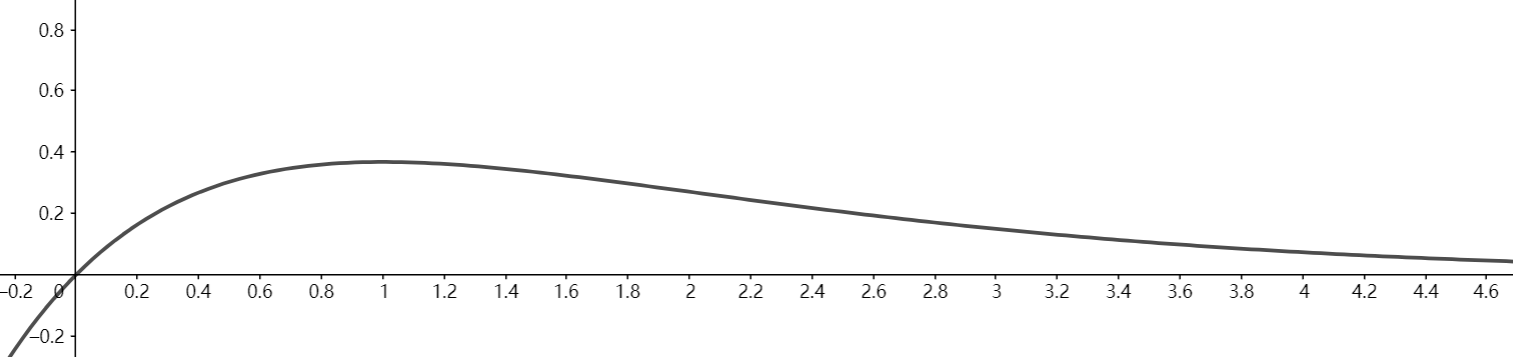
\includegraphics[scale=0.19]{picture/image1.png}
    \caption{当$n=1$的时函数的图像}
\end{figure}
\begin{figure}[htbp]
    \center
    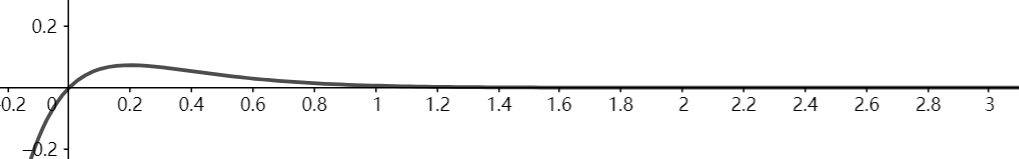
\includegraphics[scale=0.3]{picture/image2.png}
    \caption{当$n=5$的时函数的图像}
\end{figure}
你会发现这里的收敛是“均匀”的。为了更加体现这一点,我们再看一个“不那么均匀”的例子。\par
(2) $\{n^2xe^{-nx}\}_{n=1}^\infty$,$x>0$. 显然当$n\to\infty$时它也有逐点收敛于$0$,但如果我们做出它的图像(下一页图3,图4):
\begin{figure}[htbp]
    \center
    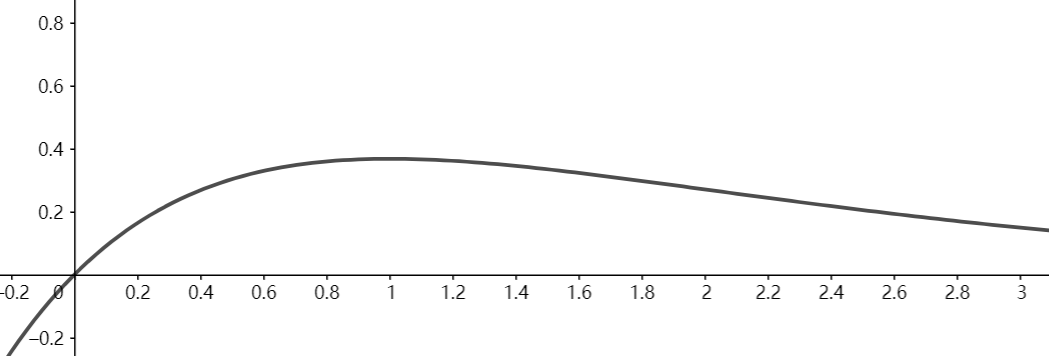
\includegraphics[scale=0.19]{picture/image3.png}
    \caption{当$n=1$的时函数的图像}
\end{figure}
\begin{figure}[htbp]
    \center
    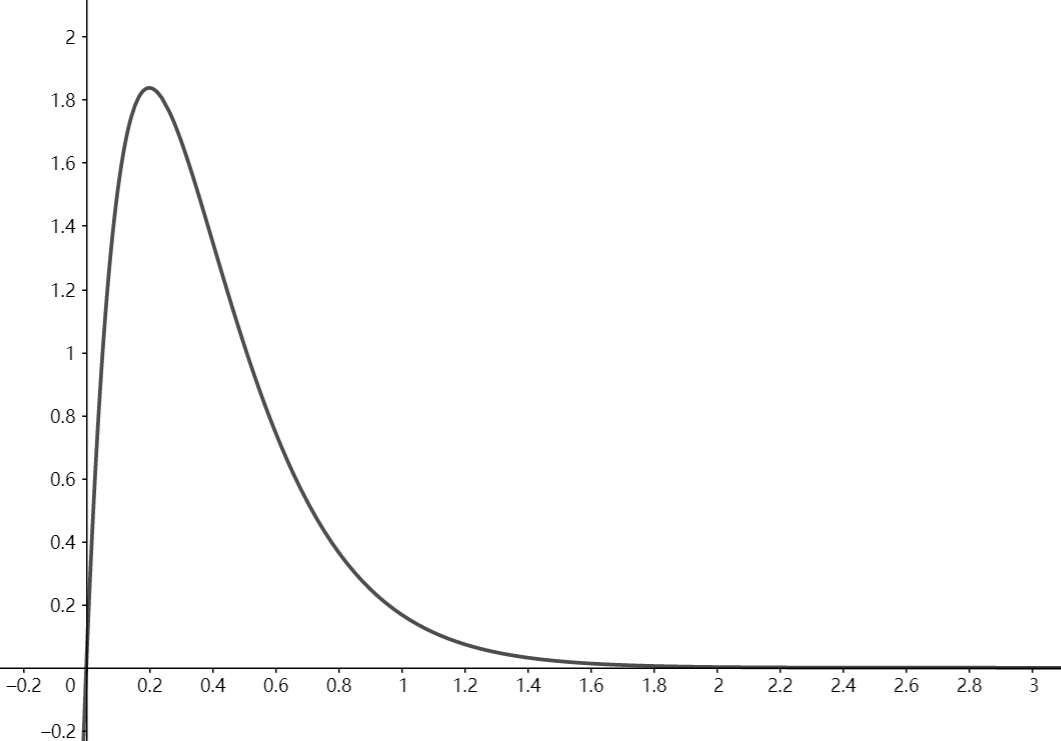
\includegraphics[scale=0.25]{picture/image4.png}
    \caption{当$n=5$的时函数的图像}
\end{figure}
这时虽然大部分地方确实收敛于$x$,但是你会发现在靠近$0$的部分有一个“凸起”,也就是说这个收敛不是“均匀”的。
\end{example}
那么我们如何刻画这种“均匀”的收敛性呢?首先从直观上,一个函数列的收敛是“均匀”的,就是对每个$x$,它的收敛情况都差不太多。这启示我们从整体上来考虑这种性质。如果对于定义域内任意的$x$都有$|S_n(x)-S(x)|<\varepsilon$,那么这样的收敛就应该是均匀的。我们给这样的收敛起一个名字:\textbf{一致收敛}(或者有些教材直接称为\textbf{均匀收敛})。\par
我们现在严格给出一致收敛的定义:
\begin{definition}
设函数列$\{f_n(x)\}$逐点收敛于$f(x)$,如果对任意的$\varepsilon>0$,存在仅与$\varepsilon$相关的常数$N_\varepsilon$,使得当$n>N_\varepsilon$时成立$|f_n(x)-f(x)|<\varepsilon$,则称$\{f_n(x)\}$\textbf{一致收敛}于$f(x)$,记作$f_n\rightrightarrows f$.
\end{definition}
如果这里的$f_n(x)$换为$S_n(x)$,$f(x)$换为$S(x)$,我们就得到了函数项级数一致收敛的定义。特别地,若函数项级数$\sum_{n=1}^\infty u_n(x)$在任意闭区间$I$上一致收敛,则称该函数项级数\textbf{内闭一致收敛},若$\sum_{n=1}^\infty|u_n(x)|$一致收敛,则称该函数项级数\textbf{绝对一致收敛}。\par
下面我们再看一个例子,请读者与例2.1.4中的例子作比较。
\begin{example}
我们考察$\{nxe^{-nx}\}_{n=1}^\infty$.我们做出它的图像(下一页图5,图6):\par
\begin{figure}[htbp]
    \center
    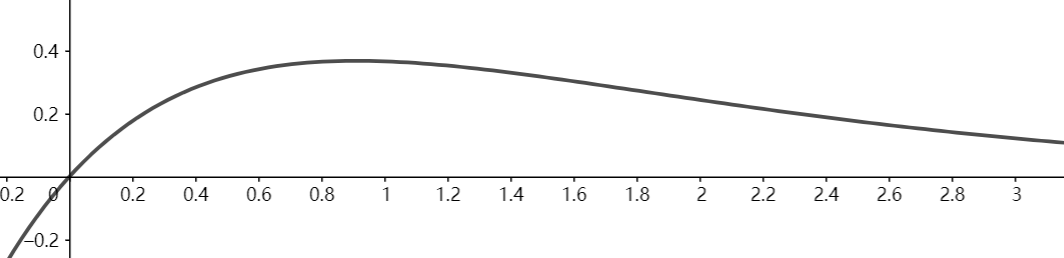
\includegraphics[scale=0.25]{picture/image5.png}
    \caption{当$n=1$的时函数的图像}
\end{figure}
\begin{figure}[htbp]
    \center
    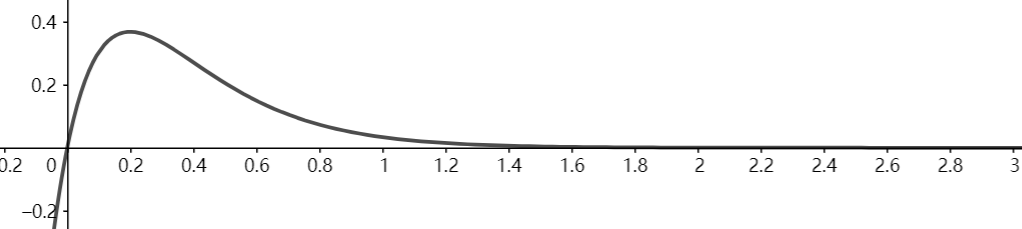
\includegraphics[scale=0.25]{picture/image6.png}
    \caption{当$n=5$的时函数的图像}
\end{figure}
读者发现它不是一致收敛的。但是相比例2.1.4中的第二个例子,它至少对每个$x$都是有界的。
\end{example}
上面的例子启发我们给出\textbf{一致有界}的定义。事实上有了一致连续的定义,下面的定义应当是自然的。
\begin{definition}
我们称函数列$\{f_n(x)\}$是一致有界的,如果存在$M>0$,使得对任意属于定义域的$x$都成立$|f_n(x)|<M$.
\end{definition}
我们将用下面一节内容来深入研究函数列的一致有界和一致收敛的概念。
\subsection{一致有界与一致收敛}
\textbf{注意:本节内容具有比较浓的{\color{red}拓扑味道},我们希望学有余力的读者学一下点集拓扑(可以参考尤承业前87页[后面是代数拓扑],随后参考Munkres学习网的语言和Baire纲定理,最后可以尝试阅读Bourbaki了解一下滤子和滤子语言下的极限),这是现代分析学的基本语言!}\par
我们在上一节中给出了逐点性质和一致性质的严格定义,下面我们来思考这样的问题:有没有什么技术,可以从逐点性质过渡到一致性质呢?我们先考虑这样一个问题:
\begin{question}
给定一个连续函数列$\{f_n(x)\}_{n=1}^\infty$,其定义域为$U$是一个区间,若对任意的$x\in U$都有$f_n(x)$有界,那么函数列$\{f_n(x)\}$\textbf{可以在多大程度上}一致有界?
\end{question}
我们首先看“对任意的$x\in U$都有$f_n(x)$有界”的条件。这句话的意思就是“存在$M\ge 0$,使得对任意的$x\in U$,都有$|f_n(x)|\le M$”.我们想用集合语言刻画这一条件。第一个问题是:\textbf{存在}如何描述?所谓“存在一个数”,就是我\textbf{遍历所有数得到的结果非空}。利用这一启示,我们可以将“存在$M\ge 0$”这一条件改写为$\bigcup_{M\ge 0}$.因此我们得到了上面条件的等价集合刻画:
$$U=\bigcup_{M\ge 0}\{x\in U:|f_n(x)|\le M,n\in\mathbb{N}_+\}.$$
现在我们希望将这一条件与一致有界联系。为此我们需要研究右面的一列集合的并的性质。一个平凡的观察是右边的集合都是闭集(注意这个函数列是连续函数列)。因此我们需要考虑\textbf{一些闭集的并能够在多大程度上继承原有的性质、能够在多大程度上带来一致的性质}?这就是下面的Baire纲定理:
\begin{theorem}(Baire)
$\mathbb{R}^n$中一列无内点的闭集的并也无内点。
\end{theorem}
\begin{proof}
后面补充
\end{proof}
\begin{note}
(1) 很显然它的一个等价表述是$\mathbb{R}^n$中一列稠密的开集的交也稠密。\par
(2) 这个定理\textbf{从局部的性质中带来了某种一致性}。我们考察上面的例子。因为$U$是一个区间,因此$U$有内点。于是根据Baire纲定理,必存在某个$M_0$使得$\{x\in U:|f_n(x)|\le M_0,n\in\mathbb{N}_+\}$有内点。取该内点的一个邻域,就得到了一个一致有界的区间。\par
(3) 对于更一般的Baire纲定理涉及到完备性的概念。感兴趣的读者可以参看张恭庆《泛函分析讲义》上册的纲与开映射定理一节。
\end{note}
下面我们来看一致有界能够带来怎样的结果。考虑一个定义在$X\subset\mathbb{R}^n$上的函数列$\{f_n\}$,它是一致有界的,即对任意的$x\in X$,存在与$x$无关的常数$M$,使得$\sup_{n\in\mathbb{N}}|f_n(x)|\le M$.如果直接就$x\in X$讨论将是困难的。这是因为我们不知道任何与$X$有关的信息。因此我们需要找一个$X$的子集,\textbf{它是具体的(也就是说,我们知道这个子集中的元素有哪些),同时它能够尽可能地刻画整个$X$的性质}。一个自然的想法是寻找$X$中的一个稠子集,因此我们需要保证这样的稠子集是存在的。这类集是重要的,于是我们人为地定义\boxed{\text{存在一个可数稠密子集的集合为一个}\textbf{可分集}}。现在我们设$X$是可分的,因此我们可以取出$X$中的一个可数稠密子集$M=\{x_1,x_2,\cdots\}$,现在我们希望从$\{f_n\}$中抽取出一列子函数列,使得新的函数列在$M$上逐点收敛。我们考察$\{f_n(x_j)\}_{n=1}^\infty$,这里$j$是某个固定的正整数,由条件知它是有界的,因此存在$\{f_{nj}\}$使得$f_{nj}(x_j)\to f(x_j)$.现在对每个$j$都这样做,我们得到下面的一张表:
$$
\begin{matrix}
	f_{11}\left( x_1 \right)&		f_{12}\left( x_1 \right)&		\cdots&		f_{1n}\left( x_1 \right)&		\cdots&		\rightarrow f\left( x_1 \right)\\
	f_{21}\left( x_2 \right)&		f_{22}\left( x_2 \right)&		\cdots&		f_{2n}\left( x_2 \right)&		\cdots&		\rightarrow f\left( x_2 \right)\\
	\vdots&		\vdots&		&		\vdots&		&		\vdots\\
	f_{m1}\left( x_m \right)&		f_{m2}\left( x_m \right)&		\cdots&		f_{mn}\left( x_m \right)&		\cdots&		\rightarrow f\left( x_m \right)\\
	\vdots&		\vdots&		&		\vdots&		&		\vdots\\
\end{matrix}
$$
现在我们选取上表中对角线上的函数构成一个新的子列:$\{f_{ii}\}_{i=1}^\infty$,那么它满足对任意的$x_i\in M$,成立$f_{nn}(x_i)\to f(x_i),n\to\infty$. 我们不妨记$f_{nn}=f_n$.为了把$f$延拓到整个空间$X$上,我们需要探索邻域信息。一个自然的想法是给$f_n$加上连续的条件,这样对任意的$x\in M$和$\varepsilon>0$,我们可以找到它的一个邻域$U_x$使得$|f_n(x)-f_n(y)|<\varepsilon$对任意的$y\in U_x$成立。我们希望说明对任意的$x\in X$都有$|f_{i}(x)-f_{j}(x)|<\varepsilon$,从而由Cauchy收敛原理就能够说明$f_n$在$X$上收敛于$f$.为了能使用连续带来的估计,我们进行如下放缩:
$$
\left| f_i\left( x \right) -f_j\left( x \right) \right|\le {\color{red} \left| f_i\left( x \right) -f_i\left( y \right) \right|}+{\color[RGB]{0, 0, 240} \left| f_i\left( y \right) -f_j\left( y \right) \right|}+{\color{red} \left| f_j\left( y \right) -f_j\left( x \right) \right|},
$$
注意到不等号右侧蓝色部分直接被连续的条件放成$\frac{\varepsilon}{3}$,只要红色部分也能被放掉,就说明了$f_i\to f$在$X$上成立。\textbf{如果这里的每个$f_n$都具有一致连续性,且这种一致连续性对函数列也一致地保持},那么两个红色的部分也就被放掉了。为此,我们再引入如下的概念:
\begin{definition}
我们称函数列\textbf{等度连续},如果对任意的$x\in X$和$\varepsilon>0$,存在$x$的某个邻域$U_x$,使得对任意的$y\in U_x$,对所有的$f_n$成立$|f_n(x)-f_n(y)|<\varepsilon$.
\end{definition}
为了我们下面的结果表述更加简洁优美,我们再引入一个概念:
\begin{definition}
我们称函数列\textbf{列紧},如果它存在一个收敛子列。
\end{definition}
根据上面的讨论,我们得到了如下的Arzela-Ascoli定理:
\begin{theorem}(Arzela-Ascoli)
一致有界且等度连续的函数族是列紧的。
\end{theorem}
其证明之轮廓已在上文中勾勒,请读者自行补充完整证明细节。
\begin{note}
这个定理在泛函分析中是重要的。事实上其逆命题也成立,即如果函数列是列紧的,那么我们有函数列一致有界且等度连续。逆命题的证明我们不介绍,感兴趣的读者可以参考张恭庆《泛函分析讲义》第二版上册第一章定理1.3.16.值得注意的是,上述“抽子列”的方法是一个非常重要的方法,例如在概率论中重要的Helly选取定理,其证明就用到了这一思想。
\end{note}
现在我们寻找逐点收敛刻画一致收敛的条件。我们将$C[0,1]$看作是一个无穷维线性空间(请读者参考楼红卫《微积分进阶》中的函数逼近定理,我们知道任意一个连续函数都可以被多项式函数逼近,因此我们可以选取$1,x,x^2,\cdots$作为它的一组无穷基),考虑$C[0,1]$的一个有穷维子空间,我们证明下面的命题:
\begin{proposition}
设$X\subset C[0,1]$是有限维子空间,那么$X$中函数列的逐点收敛蕴含一致收敛。
\end{proposition}
\begin{proof}
由于$X$是有限维子空间,我们取它的一个基$f_1,f_2,\cdots,f_m$,我们设$f^{(k)}(x)=\sum_{i=1}^mc_i^{(k)}f_i(x)$,且$\lim_{k\to\infty}f^{(k)}(x)=f(x)$对任意的$x\in X$都成立。我们首先证明如下的引理:
\begin{lemma}
函数列$f_1,f_2,\cdots,f_m$线性无关的充要条件是存在$x_1,x_2,\cdots,x_m$使得
$$
\left| \begin{matrix}
	f_1\left( x_1 \right)&		f_1\left( x_2 \right)&		\cdots&		f_1\left( x_m \right)\\
	f_2\left( x_1 \right)&		f_2\left( x_2 \right)&		\cdots&		f_2\left( x_m \right)\\
	\vdots&		\vdots&		&		\vdots\\
	f_m\left( x_1 \right)&		f_m\left( x_2 \right)&		\cdots&		f_m\left( x_m \right)\\
\end{matrix} \right|\ne 0.
$$
\end{lemma}
现在我们证明上面的引理。充分性是容易的。我们令$f(x)=\sum_{i=1}^mc_if_i(x)$,并分别令$x=x_i,i=1,2,\cdots,m$,我们得到如下的线性方程组:
$$
\begin{cases}
	c_1f_1\left( x_1 \right) +c_1f_1\left( x_2 \right) +\cdots +c_1f_1\left( x_m \right) =0;\\
	c_2f_2\left( x_1 \right) +c_2f_2\left( x_2 \right) +\cdots +c_2f_2\left( x_m \right) =0;\\
	\vdots\\
	c_mf_m\left( x_1 \right) +c_mf_m\left( x_2 \right) +\cdots +c_mf_m\left( x_m \right) =0;\\
\end{cases}
$$
将$c_i$看作未知数,我们发现其系数矩阵对应的行列式不等于$0$,因此线性方程组有非零解,从而$f_1,f_2,\cdots,f_m$线性无关。反之,我们用归纳法证明。设在$k-1$时我们有
$$
\left| \begin{matrix}
	f_1\left( x_1 \right)&		f_1\left( x_2 \right)&		\cdots&		f_1\left( x_{k-1} \right)\\
	f_2\left( x_1 \right)&		f_2\left( x_2 \right)&		\cdots&		f_2\left( x_{k-1} \right)\\
	\vdots&		\vdots&		&		\vdots\\
	f_{k-1}\left( x_1 \right)&		f_{k-1}\left( x_2 \right)&		\cdots&		f_{k-1}\left( x_{k-1} \right)\\
\end{matrix} \right|\ne 0,
$$
考虑
$$
\left| \begin{matrix}
	f_1\left( x_1 \right)&		f_1\left( x_2 \right)&		\cdots&		f_1\left( x \right)\\
	f_2\left( x_1 \right)&		f_2\left( x_2 \right)&		\cdots&		f_2\left( x \right)\\
	\vdots&		\vdots&		&		\vdots\\
	f_k\left( x_1 \right)&		f_k\left( x_2 \right)&		\cdots&		f_k\left( x \right)\\
\end{matrix} \right|
$$
按最后一列展开得到的函数$f\left( x \right) =\sum_{i=1}^k{\left( -1 \right) ^if_i\left( x \right) \det A_i}$,其中$\det A_i$为按第$i$行的元素展开得到的余子式。由于$f_1,f_2,\cdots,f_k$线性无关,因此$f$不恒等于$0$,从而存在$x_k$使得
$$
\left| \begin{matrix}
	f_1\left( x_1 \right)&		f_1\left( x_2 \right)&		\cdots&		f_1\left( x_k \right)\\
	f_2\left( x_1 \right)&		f_2\left( x_2 \right)&		\cdots&		f_2\left( x_k \right)\\
	\vdots&		\vdots&		&		\vdots\\
	f_k\left( x_1 \right)&		f_k\left( x_2 \right)&		\cdots&		f_k\left( x_k \right)\\
\end{matrix} \right|\ne 0.
$$
利用归纳法我们完成了证明。\par
下面我们回到原题。由题意知我们有如下的线性方程组:
$$
\left( \begin{matrix}
	f_1\left( x_1 \right)&		f_2\left( x_1 \right)&		\cdots&		f_m\left( x_1 \right)\\
	f_1\left( x_2 \right)&		f_2\left( x_2 \right)&		\cdots&		f_m\left( x_2 \right)\\
	\vdots&		\vdots&		&		\vdots\\
	f_1\left( x_m \right)&		f_2\left( x_m \right)&		\cdots&		f_m\left( x_m \right)\\
\end{matrix} \right) \left( \begin{array}{c}
	c_{1}^{\left( k \right)}\\
	c_{2}^{\left( k \right)}\\
	\vdots\\
	c_{m}^{\left( k \right)}\\
\end{array} \right) =\left( \begin{array}{c}
	f^{\left( k \right)}\left( x_1 \right)\\
	f^{\left( k \right)}\left( x_2 \right)\\
	\vdots\\
	f^{\left( k \right)}\left( x_m \right)\\
\end{array} \right) .
$$
由前面的引理知
$$
\left( \begin{array}{c}
	c_{1}^{\left( k \right)}\\
	c_{2}^{\left( k \right)}\\
	\vdots\\
	c_{m}^{\left( k \right)}\\
\end{array} \right) =\left( \begin{matrix}
	f_1\left( x_1 \right)&		f_2\left( x_1 \right)&		\cdots&		f_m\left( x_1 \right)\\
	f_1\left( x_2 \right)&		f_2\left( x_2 \right)&		\cdots&		f_m\left( x_2 \right)\\
	\vdots&		\vdots&		&		\vdots\\
	f_1\left( x_m \right)&		f_2\left( x_m \right)&		\cdots&		f_m\left( x_m \right)\\
\end{matrix} \right) ^{-1}\left( \begin{array}{c}
	f^{\left( k \right)}\left( x_1 \right)\\
	f^{\left( k \right)}\left( x_2 \right)\\
	\vdots\\
	f^{\left( k \right)}\left( x_m \right)\\
\end{array} \right) ,
$$
从而我们可以解出每个$c_i^{(k)}$.而每个$f^{(k)}(x_i)$收敛,故存在$c_i$使得$c_i^{(k)}\to c_i$,因此
$$
\left| f^{\left( k \right)}\left( x \right) -f\left( x \right) \right|=\left| \sum_{j=1}^m{\left( c_{j}^{\left( k \right)}-c_j \right) f_k\left( x \right)} \right|\le \sum_{j=1}^m{\left| c_{j}^{\left( k \right)}-c_j \right|\cdot \left| f_k\left( x \right) \right|}\le \mathop {\mathrm{sup}} \limits_{x\in X,k=1,2,\cdots ,m}\left| f_k\left( x \right) \right|\cdot \sum_{j=1}^m{\left| c_{j}^{\left( k \right)}-c_j \right|}\rightarrow 0,
$$
上述收敛是独立于$x$的取值的。
\end{proof}
\subsection{函数项级数的一致收敛判别法}
我们在前面已经说过,研究函数项级数的性质,本质上就是在研究它的部分和函数$S_n(x)$所构成的函数列$\{S_n(x)\}_{n=1}^\infty$的性质。因此我们首先先探究函数列的一致收敛的充要条件。在给出正式的定理之前,我们先来算几个例子。
\begin{example}
回忆我们引入一致收敛概念时举出的例子$\{n^\alpha xe^{-nx}\}$.我们现在想通过计算来严格说明我们上一节提到的直觉。我们利用软件发现函数项级数$\{xe^{-nx}\}$应当是一致收敛于$0$的。也就是说,对任意的$\varepsilon>0$,存在某个仅与$\varepsilon$有关的常数$N_\varepsilon$,使得当$n>N$时成立$|f_n(x)|<\varepsilon$.让我们来考虑$|f_n(x)|$.我们不妨直接把它放成最大值。注意到
$$
f_{n}^{\prime}\left( x \right) =e^{-nx}-nxe^{-nx}=\left( 1-nx \right) e^{-nx},
$$
因此当$x=\frac{1}{n}$时$|f_n(x)|$取最大值$\frac{1}{ne}$.令$n\to\infty$,显然$|f_n(x)|\to 0$.\par
现在我们来看更一般的$\{n^\alpha xe^{-nx}\}$的情形。显然它们也收敛于$0$,但是如果我们计算$|f_n(x)|$的最大值,我们有$|f_n(x)|\le\frac{n^{\alpha-1}}{e}$.此时$\{f_n\}$的收敛情况已经明朗了。
\end{example}
上面的例子表明,很多时候利用定义,再加上一定的放缩技巧,就已经可以处理很多一致收敛的问题了。事实上在上面的例子里,我们已经隐含地用到了如下的定理:
\begin{theorem}
设函数列$\{f_n(x)\},x\in I$逐点收敛于$f$,那么$\{f_n(x)\}$一致收敛于$f$当且仅当
$$\beta_n=\sup_{x\in I}|f_n(x)-f(x)|\to 0.$$
\end{theorem}
\begin{proof}
设$f_n$一致收敛于$f$,那么对任意$\varepsilon>0$,对充分大的$n$成立$|f_n(x)-f(x)|<\varepsilon$,进而对充分大的$n$成立$\beta_n=\sup_{i\in I}|f_n(x)-f(x)|<\varepsilon$.反之我们有$|f_n(x)-f(x)|\le\sup_{i\in I}|f_n(x)-f(x)|\to 0$.
\end{proof}
类比数列的Cauchy收敛准则,我们还有函数列的Cauchy收敛准则:
\begin{theorem}(Cauchy)
设函数列$\{f_n(x)\},x\in I$逐点收敛于$f$,那么$\{f_n(x)\}$一致收敛于$f$当且仅当对任意的$\varepsilon>0$,存在仅与$\varepsilon$相关的$N$使得当$n>N$时成立
$$|f_n(x)-f_{n+p}(x)|<\varepsilon,\forall p\in\mathbb{N}_+.$$
\end{theorem}
\begin{proof}
设$f_n$一致收敛于$f$,那么
$$|f_n(x)-f_{n+p}(x)|\le|f_n(x)-f(x)|+|f(x)-f_{n+p}(x)|<\frac{\varepsilon}{2}+\frac{\varepsilon}{2}=\varepsilon.$$
反之,令$p\to\infty$.
\end{proof}
利用上面的定理,我们很容易得到函数项级数的一致收敛判别法:
\begin{corollary}
设$\sum_{n=1}^\infty u_n(x)$是逐点收敛的函数项级数,那么$\sum_{n=1}^\infty u_n(x)$是一致收敛的当且仅当它的部分和一致收敛。
\end{corollary}
上述推论的证明是平凡的,我们略去。我们回忆在上一节讲的控制收敛定理中对于充分大项的估计,在那时我们指出,为了能够安全地放掉充分大项,只要能找到一个控制函数即可。而在这里我们注意到,对于$\sum_{k=n+1}^{n+p}u_k(x)$,如果我们能找到一个控制级数$\sum M_n$,那么
$$\left|\sum_{k=n+1}^{n+p}u_n(x)\right|\le\sum_{k=n+1}^{n+p}|u_n(x)|\le\sum_{k=n+1}^{n+p}|M_k|\to 0,$$
从而我们得到如下的\textbf{优级数判别法}:
\begin{theorem}
如果存在收敛的正项级数$\sum_{n=1}^\infty a_n$,使得对任意的$x$和$n$都成立$|u_n(x)|\le a_n$,那么$\sum_{n=1}^\infty u_n(x)$一致收敛。
\end{theorem}
证明只要利用上面给出的估计。
\begin{example}
我们考察级数$\sum_{n=1}^\infty ne^{-nx}$. 如果我们考虑$x\in(0,+\infty)$, 那么事实上这个级数不是一致收敛的。这是因为显然它的通项收敛于$0$,但
$$
\mathop {\mathrm{sup}} \limits_{x\in \left( 0,+\infty \right)}\left| u_n\left( x \right) \right|\ge \left| u_n\left( \frac{1}{n} \right) \right|=\frac{n}{e}\rightarrow +\infty ,
$$
因此通项不是一致收敛的。但若我们取$\delta>0$并考虑$[\delta,+\infty)$,那么这个级数是一致收敛的。这是因为对充分大的$n$,我们有
$$
0<ne^{-nx}<ne^{-n\delta}<\frac{1}{n^2},
$$
而$\sum\frac{1}{n^2}<\infty$,由优级数判别法就说明了一致收敛性。
\end{example}
我们最后不加证明地(证明是容易的,读者可以仿照数项级数中的AD判别法给出证明)给出下面两个判别法:
\begin{theorem}(Dirichlet)
如果函数项级数$\sum_{n=1}^\infty a_n(x)b_n(x)$满足:\par
(1)$\{b_n(x)\}$对每个固定的$x\in I\subset\mathbb{R}$都是单调的,且在$I$上一致收敛于$0$;\par
(2)$\sum_{n=1}^\infty a_n(x)$的部分和在$I$上一致有界,\par
那么$\sum_{n=1}^\infty a_n(x)b_n(x)$在$I$上一致收敛。
\end{theorem}
\begin{theorem}(Abel)
如果函数项级数$\sum_{n=1}^\infty a_n(x)b_n(x)$满足:\par
(1)$\{b_n(x)\}$对每个固定的$x\in I\subset\mathbb{R}$都是单调的,且在$I$上一致有界;\par
(2)$\sum_{n=1}^\infty a_n(x)$一致收敛,\par
那么$\sum_{n=1}^\infty a_n(x)b_n(x)$在$I$上一致收敛。
\end{theorem}
\newpage
\section*{后记:一个求和与Fourier分析}
由于时间有限,我们不可能很深入的讨论级数中的一些有趣的问题,对于一些我们没有提到但仍然重要的内容,我们把它们写在后记里,并附上一些参考书,供感兴趣的读者查阅。\par
虽然大多数数分教材在讲级数的时候都会捎带着提一些Fourier级数的内容,但调和分析(Fourier分析)本身也是值得我们深入了解的。我们举一例计算数项级数的例子:
\begin{example}
计算$\sum_{m\in\mathbb{Z}}e^{-m^2t}$,这里$t$是正的常数。
\end{example}
如果直接利用初等方法计算,难度很大。但如果我们引入下面调和分析中的定理:
\begin{theorem}
设$f(x)\in C(\mathbb{R})$,且存在$C,\delta>0$使得$|f(x)|<\frac{C}{(1+|x|)^{1+\delta}}$,记$\widehat{f}(x)$为$f$的Fourier展开,且$\sum_{m\in\mathbb{Z}}|\widehat{f}(m)|<\infty$,那么
$$
\sum_{m\in \mathbb{Z}}{\widehat{f}\left( m \right) e^{2\pi \mathrm{i}mx}}=\sum_{m\in \mathbb{Z}}{f\left( x+m \right)}.
$$
\end{theorem}
我们就可以对上述例子中的级数做如下计算:
\begin{proof}
令$a=-2\pi\mathrm{i}x$,注意到
$$
\int_{-\infty}^{+\infty}{e^{-ty^2}e^{ay}\mathrm{d}y}=e^{\frac{a^2}{4t}}\int_{-\infty}^{+\infty}{e^{-t\left( y-\frac{a}{2t} \right) ^2}\mathrm{d}y}=\frac{1}{\sqrt{t}}e^{\frac{a^2}{4t}}\int_{-\infty}^{+\infty}{e^{-y^2}\mathrm{d}y}=\sqrt{\frac{\pi}{t}}e^{-\frac{\pi ^2x^2}{t}},
$$
因此
$$
\sum_{m\in \mathbb{Z}}{e^{-tm^2}}=\sum_{m\in \mathbb{Z}}{f\left( m \right)}=\sum_{m\in \mathbb{Z}}{\widehat{f}\left( m \right)}=\sqrt{\frac{\pi}{t}}\sum_{m\in \mathbb{Z}}{e^{-\frac{\pi ^2x^2}{t}}}.
$$
\end{proof}
上面的定理叫做Possion求和公式,关于证明读者可以参考GTM249(古典调和分析)中的定理3.2.8.一般而言,一些比较进阶的实变函数书(比如Rudin,Folland)和泛函分析中会有一点点关于Fourier分析的讨论。读者若想深入学习调和分析,GTM249是不错的入门书。
\newpage
\end{document}
